%% LyX 2.3.6.1 created this file.  For more info, see http://www.lyx.org/.
%% Do not edit unless you really know what you are doing.
\documentclass[english]{article}
\usepackage[T1]{fontenc}
\usepackage[latin9]{inputenc}
\usepackage{array}
\usepackage{multirow}
\usepackage{amsmath}
\usepackage{amsthm}
\usepackage{amssymb}
\usepackage{graphicx}

\makeatletter

%%%%%%%%%%%%%%%%%%%%%%%%%%%%%% LyX specific LaTeX commands.
%% Because html converters don't know tabularnewline
\providecommand{\tabularnewline}{\\}

%%%%%%%%%%%%%%%%%%%%%%%%%%%%%% Textclass specific LaTeX commands.
\numberwithin{equation}{section}
\numberwithin{figure}{section}
\usepackage[natbibapa]{apacite}
\theoremstyle{plain}
\newtheorem{thm}{\protect\theoremname}
\theoremstyle{definition}
\newtheorem{defn}[thm]{\protect\definitionname}
\theoremstyle{definition}
\newtheorem{example}[thm]{\protect\examplename}
\theoremstyle{plain}
\newtheorem{lem}[thm]{\protect\lemmaname}
\theoremstyle{plain}
\newtheorem{prop}[thm]{\protect\propositionname}

%%%%%%%%%%%%%%%%%%%%%%%%%%%%%% User specified LaTeX commands.
\usepackage{kappa-sd-with-name}

\titletag{Submitted manuscript}
\makeatletter
\titlerunning{\@title}
\makeatother
\authorrunning{Jonas Moss}

\usepackage{booktabs}
% \renewcommand{\sqrt}[1]{{(#1)^{1/2}}}
\DeclareMathOperator{\tr}{tr}
\DeclareMathOperator{\Tr}{Tr}
\DeclareMathOperator{\Var}{Var}
\DeclareMathOperator{\sd}{sd}
\DeclareMathOperator{\argmin}{argmin}
\DeclareMathOperator{\Cor}{Cor}
\DeclareMathOperator{\Cov}{Cov}
\DeclareMathOperator{\diag}{diag} 
\DeclareMathOperator{\se}{se} 
\DeclareMathOperator{\argmax}{argmax}
\DeclareMathOperator{\artanh}{artanh}
\DeclareMathOperator{\supp}{supp}

\usepackage{enumitem}
\setlist[enumerate]{label = (\roman*)}

\makeatother

\usepackage{babel}
\providecommand{\definitionname}{Definition}
\providecommand{\examplename}{Example}
\providecommand{\lemmaname}{Lemma}
\providecommand{\propositionname}{Proposition}
\providecommand{\theoremname}{Theorem}

\begin{document}
\title{Inference for measures of agreement with multiple raters}
\author{Jonas Moss \orcid{0000-0002-6876-6964}\\
Department of Data Science and Analytics\\
BI Norwegian Business School\emph{}\\
\emph{jonas.moss@bi.no}}
\maketitle
\begin{abstract}
Most measures of agreement are chance-corrected measures of agreement.
They differ in three dimensions: their definition of chance agreement,
their choice of disagreement function, and how they handle multiple
raters. Chance agreement is usually defined following either Cohen's
kappa or Fleiss' kappa. The disagreement function is usually either
the nominal, quadratic, or the absolute value function. But how to
handle multiple raters is contentious, with the main contenders being
Fleiss' kappa, Conger's kappa, and Hubert's kappa, the variant of
Fleiss' kappa where agreement is only said to occur if every rater
agrees. More generally, multi-rater agreement coefficients can be
defined in a $g$-wise way, where the disagreement weighting function
uses $g$ of the raters. This paper contains two main contributions.
(a) We propose to use Fr�chet variances to handle the case of multiple
raters. The Fr�chet variances are intuitive disagreement measures,
and turn out to generalize the nominal, quadratic, and absolute value
functions to the case of more than 2 raters. (b) We derive the limit
theory of $g$-wise weighted agreement coefficients, with chance agreement
either of the Cohen type or Fleiss type, for the case when every item
is rated by the same number of raters. Trying out three confidence
interval constructions, we end up recommending to calculate confidence
intervals using the arcsine transform or the Fisher transform.
\end{abstract}

\section{Introduction}

Most popular measures of inter-rater agreement involve correction
for chance agreement. These can be written on the form 
\begin{equation}
\frac{p_{a}-p_{ca}}{1-p_{ca}}=1-\frac{p_{d}}{p_{cd}},\label{eq:chance-corrected measure of agrement}
\end{equation}
where $p_{a}$ ($p_{d}$) is the percent agreement (disagreement)
between the raters and $p_{ca}$ ($p_{cd}$) is the chance agreement
(disagreement) between the raters. Such measures are frequently called
\emph{chance-corrected measures of agreement}. Well-known examples
of coefficients in this class are Cohen's \citeyearpar{Cohen1960-mp}
kappa and its weighted variant \citeyearpar{Cohen1968-sb}, Krippendorff's
\citeyearpar{Krippendorff1970-gl} alpha, Scott's \citeyearpar{Scott1955-vn}
pi, and Fleiss' \citeyearpar{Fleiss1971-to} kappa. Some of these
coefficients are either defined only for two raters. The rest are
defined in a pairwise manner, in the sense they measure agreement
between two raters at a time. But not every proposed measure of agreement
is defined on pairs of raters. The most famous is Hubert's kappa \citeyearpar{Hubert1977-ox},
which was recently studied in detail by \citet{Martin_Andres2020-jr}.
Other two-rater agreement coefficients include Conger's kappa \citep{Conger1980-yx,Light1971-ad},
which is Cohen's kappa generalized to multiple raters, the $AC_{1}$
coefficient \citep{Gwet2008-qk}, and the recent coefficient of \citet{Van_Oest2019-pm}.

There is no consensus about how multi-rater agreement coefficients
should be defined. Broadly speaking, there are two options, pairwise
coefficients and consensus coefficients. Pairwise coefficients measure
agreement between pairs of raters \citep{Conger1980-yx}, while consensus
coefficients measure the simultaneous agreement between all raters.
In particular, consensus coefficients support the notion that ``agreement
occurs if and only if all raters agree on the categorization of an
object'' \citep{Hubert1977-ox}. Both pairwise and consensus-based
definitions of agreement are variants of $g$-wise measures of agreement
\citep{Conger1980-yx}, where agreement is measured among $g$-tuples
of raters. But not-trivial ways to measure agreement is hard to come
by when $2<g<R$. In Section \ref{sec:Fr=0000E9chet-variances} we
introduce a framework for handling $g$-wise measures on agreement
based on the concept of \emph{Fr�chet variances }\citep{Dubey2019-rh}.
The Fr�chet variances, based on the Fr�chet mean, generalize the variance,
and the measures of agreement based on them generalize the nominal,
linearly weighted, and quadratically weighted pairwise measures of
agreement in a natural way. They are easily interpretable as, you
measure how much do the raters disagree with the (generalized) mean
rater, and then adjust for chance. For nominal data in particular,
they measure how many raters disagree with the modal rater, with a
resulting agreement measure less extreme than Hubert's kappa \citep{Hubert1977-ox}. 

Assuming multivariate normality of the judgments, \citet[Section 3]{Lin1989-kf}
derived the asymptotic distribution of Cohen's kappa with quadratic
weights. \citet{Fleiss1971-to} introduced a formula for the standard
error of Fleiss' kappa, but later showed that it was incorrect. Using
the properties of the multinomial distribution and the delta method,
\citet{Schouten1982-ou} found the asymptotic variance of the weighted
Fleiss' kappa in the case when the number of categories is finite.
Almost forty years later, \citet{Gwet2021-ht} found a consistent
estimator of the variance for the unweighted Fleiss' kappa. We extend
these results to the weighted $g$-wise Fleiss' kappa for any number
of categories below. In addition, we mention that bootstrap inference
for Fleiss' kappa and Krippendorff's alpha was studied by \citet{Zapf2016-eu}.

We begin the paper by providing the definitions of two kinds of chance-corrected
agreement coefficients, then we establish connections between a multi-rater
weighted Cohen's kappa, the weighted Fleiss' kappa, Conger's kappa,
Krippendorff's alpha, and Hubert's kappa (Section \ref{sec:Pairwise-kappa-like-statistics}).
We restrict ourselves to the simple context when every rater rates
every item. In Section \ref{sec:Fr=0000E9chet-variances} we introduce
the Fr�chet variances, a useful class of disagreement functions that
make sense when $2<g<R$. Then we spell out the basic limit theory
for this class agreement coefficients (Section \ref{sec:Estimation}),
extending the results of \citet{Schouten1980-iv}, \citet{Schouten1982-ou}
and \citet{OConnell1984-dz} to vector-valued items and $g$-wise
coefficients. We do this using $U$-statistics \citep{Lee2019-xm},
but there are other ways to arrive at the same results. Then we provide
practical recommendations regarding the choice of confidence interval
construction, obtained by comparing three confidence interval constructions:
basic, arcsine transformed, and Fisher transformed. Using a simulation
study (Section \ref{sec:Simulation-of-confidence-k2}), we find that
the arcsine and Fisher intervals outperform the basic interval when
$n$ is small.

\section{Measures of agreement\label{sec:Pairwise-kappa-like-statistics}}

Discussing measures of inter-rater agreement requires quite a few
definitions. Let $d(x_{1},\ldots,x_{g})$ be a\emph{ disagreement
function}, a positive and symmetric function of $g$ arguments that
equals $0$ when all $x_{i}$s are equal, i.e., $d(x,\ldots,x)=0$.
This function measures the disagreement between the judgments $x_{1},\ldots,x_{k}$,
where $0$ is understood as complete agreement. 

All disagreement functions in widespread use take two arguments. While
there are infinitely many disagreement functions, the best known belong
to the class of $l_{p}$ quasi-norms, $p=0,1,2$, potentially raised
to the $p$th power. The $l_{p}$ quasi-norms, $p\in[0,\infty]$ on
$\mathbb{R}^{g}$ are defined as
\begin{equation}
\|x\|_{p}=(\sum_{i=1}^{g}|x_{i}|^{p})^{1/p}.\label{eq:d_p_definitio}
\end{equation}
Here $||x||_{0}=\sum_{i=1}^{g}1[x_{i}\neq0]$ and $||x||_{\infty}=(\sum_{i=1}^{g}|x_{i}|^{p})^{1/p}$,
as can be verified by taking the limit of $||x||_{p}$ as $p\to0$
and $p\to\infty$, respectively. It is well known that $||x||_{p}$
are proper norms if and only if $p\geq1$, as the triangle inequality
is violated when $1>p\geq0$. 

Define the disagreement functions $d_{p}$ as the $l_{p}$-norm evaluated
in $x_{1}-x_{2}$, i.e.,
\begin{equation}
d_{p}(x_{1},x_{2})=||x_{1}-x_{2}||_{p}.\label{eq:d_p}
\end{equation}
In the case of scalar values, $d_{0}(x_{1},x_{2})=1[x_{1}\neq x_{2}]$
is known as the \emph{nominal disagreement function}. For $p=1$,
the $l_{p}$-norm equals $d_{1}(x_{1},x_{2})=|x_{1}-x_{2}|$, which
is known as the \emph{absolute value disagreement function} (and sometimes
the linear disagreement function). The \emph{quadratic disagreement
function} is $d_{2}^{2}(x_{1},x_{2})=(x_{1}-x_{2})^{2}$. Vector-valued
variants of $d_{p}$ and $d_{p}^{p}$ are far less common, but have
been used by e.g. \citet{Berry2008-ga}

When the dimension of $d$ isn't equal to $2$, we are mostly interested
in the case when its arty equals the number of raters $R$. In this
case, the disagreement functions often measure the degree of consensus
among the raters, with $0$ reflecting complete consensus. The most
obvious choice is the Hubert disagreement function
\begin{equation}
d(x_{1},\ldots,x_{K})=1-1[x_{1}=\cdots=x_{K}]\label{eq:Hubertweight}
\end{equation}
which equals $0$ if and only if every rater agrees on a rating. It
is the disagreement function employed in Hubert's kappa \citep{Hubert1977-ox}.
This is not the only reasonable disagreement function for multiple
raters, however. We will come back to that in Section \ref{sec:Fr=0000E9chet-variances}.

We present our results in terms of disagreement functions instead
of the more popular agreement functions (i.e., positive functions
bounded by $1$ where $1$ signifies maximal agreement, sometimes
with the additional assumption that $a\geq0$). We do this mainly
for mathematical convenience. Agreement functions and disagreement
functions are tightly related, for if $a$ is an agreement function
then $d=1-a$ is a disagreement function. See the appendix, p. \pageref{subsec:Agreement-vs-disagreement}
for a more detailed discussion.

Let $R$ denote the number of raters and $n$ denote the numbers of
items rated. We make several assumptions. First, we assume that the
ratings are conditionally independent given the item. Second, we assume
that every item is rated by exactly the same number of raters, which
we refer to as the \emph{rectangular design}, which is common in the
literature. \footnote{For instance, \citet{Fleiss1971-to}, in his paper introducing Fleiss'
kappa, removed several ratings from this data to make sure the total
number of ratings was $6$ for each item.} The rectangular design assumption can be relaxed, but it is needed
for the limit results. We sketch how to loosen it up in the appendix
(p. \pageref{subsec:Expanding-the-definitions}). Third, we will assume
either: (a) Fixed raters, so the same set of raters rate every item,
most commonly associated with applications of Cohen's kappa, or (b)
Exchangeable ratings given the item, which is the case when the ratings
are independent and identically distributed conditional on the item
rater, an implicit assumption underlying most applications of Fleiss'
kappa, e.g., \citep{Fleiss1971-to}. In case (b), the marginal distributions
for all raters will be equal, which implies that the population value
of the Fleiss' kappa equals the population value of the generalized
Cohen's kappa, both defined below. But the sample Fleiss' kappa is
the preferred sample estimator, as it is invariant under changes of
the raters' identities. 

We will also assume that the ratings are made independently of one
another in the sense the ratings on the $i$th item in no way affects
the ratings on $k$th item. This situation corresponds to a statistical
model where $\boldsymbol{X}_{1},\boldsymbol{X}_{2},...,\boldsymbol{X}_{n}$,
$R$-dimensional vectors (whose elements may also be vectors) are
sampled independently from some distribution $F$. Be aware that we
\emph{do not} assume that $\boldsymbol{X}_{k}$ contains only categorical
values, or a finite number of values; the elements of $\boldsymbol{X}_{k}$
are arbitrary in our framework.

Our intention is to collect the kappas of Cohen, Fleiss, Conger, Hubert,
and so on, into a coherent framework of $g$-wise agreement coefficients.
To do this we will have to define some quantities. Let $\boldsymbol{x}_{i}=(x_{i1},x_{i2},\ldots,x_{iR})$
be an $R$-dimensional vector of observed ratings and recall that
$g$ is the dimension of our disagreement function $d$. 
\begin{enumerate}
\item \textbf{The disagreement $\boldsymbol{x}_{1}$,} as measured by $d$.
The purpose of this quantity is to translate an arbitrary $g$-dimensional
disagreement function $d$ into a disagreement function taking an
$R$-dimensional vector $\boldsymbol{x}_{i}$ as input. It is defined
as
\begin{equation}
D_{d}(\boldsymbol{x}_{1})=\binom{R}{g}^{-1}\sum_{j_{i}}d(\boldsymbol{x}_{1j_{1}},\ldots,\boldsymbol{x}_{1j_{g}}),\label{eq:D_d}
\end{equation}
where the sum runs over all $g$-dimensional subsets of $\{1,\ldots,R\}$
with order ignored, i.e., the $g$-combinations of $R$. The expression
is simplified when $g=R$, as $D_{d}(\boldsymbol{x}_{1})=d(\boldsymbol{x}_{11},\ldots,\boldsymbol{x}_{1R})$
in this case. To gain some intuition about this quantity, suppose
that $g=2$, that $x_{1},x_{2}$ are scalars, and consider the nominal
disagreement function $d_{0}(x_{1},x_{2})=1[x_{1}\neq x_{2}]$. Then
$D_{d}(\boldsymbol{x}_{1})=2R^{-1}(R-1)^{-1}\sum_{j_{1}>j_{2}}1[x_{1j_{1}}\neq x_{1j_{2}}]$
is the percentage of times two raters precisely agree on their rating.
\item \textbf{The Cohen-type chance disagreement} at $\boldsymbol{x}_{1},...,\boldsymbol{x}_{g}$,
so called to differentiate it from the Fleiss-type chance disagreement.
It is similar to the disagreement at $\boldsymbol{x}_{1}$, but this
time the raters do not necessarily rate the same item, as one rater
raters the first item (from $\boldsymbol{x}_{1}$) another rater raters
the second item (from $\boldsymbol{x}_{2}$), and so on. We do not
allow a rater to rate the same item more than once in a pass: Hence
we need to choose $g$ raters from a set of $R$ raters, and the chance
disagreement is
\begin{equation}
C_{d}(\boldsymbol{x}_{1},...,\boldsymbol{x}_{g})=\binom{R}{g}^{-1}\sum_{j_{i}}d(\boldsymbol{x}_{1j_{1}},\ldots,\boldsymbol{x}_{gj_{g}}),\label{eq:C_d}
\end{equation}
where the sum runs over all $g$-dimensional subsets of $\{1,\ldots,R\}$,
i.e., the $g$-combinations of $R$. Observe that $D_{d}(\boldsymbol{x})=C_{d}(\boldsymbol{x},,\ldots,\boldsymbol{x})$.
Since $d$ is assumed to be symmetric, the expression is massively
simplified to $d(\boldsymbol{x}_{1j_{1}},\ldots,\boldsymbol{x}_{Rj_{R}})$
when $g=R$. When $g=2$, $C_{d}(\boldsymbol{x}_{1},\boldsymbol{x}_{2})=R^{-1}(R-1)^{-1}\sum_{j_{1}\neq j_{2}}d(\boldsymbol{x}_{1j_{1}},\boldsymbol{x}_{2j_{2}})$.
\item \textbf{The Fleiss-type chance disagreement} at $\boldsymbol{x}_{1},...,\boldsymbol{x}_{g}$
is similar, but allows the same rater (or rater index) to rate an
item multiple times. Its definition is 
\[
F_{d}(\boldsymbol{x}_{1},...,\boldsymbol{x}_{g})=R^{-g}\sum_{j_{i}}d(\boldsymbol{x}_{1j_{1}},\ldots,\boldsymbol{x}_{gj_{g}}),
\]
where the sum runs over the product set $R^{g}$. The expression for
$F_{w}(\boldsymbol{x}_{1},...,\boldsymbol{x}_{g})$ is not dramatically
simplified when $g=R$. When $g=2$, $F_{d}(\boldsymbol{x}_{1},\boldsymbol{x}_{2})=R^{-2}\sum_{j_{1},j_{2}}d(\boldsymbol{x}_{1j_{1}},\boldsymbol{x}_{2j_{2}})$.
\end{enumerate}
We will call the expected values of these quantities the \emph{mean
disagreement}, the \emph{mean Cohen-type chance disagreement}, and
the \emph{mean Fleiss-type chance disagreement}. Slightly abusing
notation, we denote them as
\begin{equation}
D_{d}=E[D_{d}(\boldsymbol{X}_{1})],\quad C_{d}=E[C_{d}(\boldsymbol{X}_{1},\ldots,\boldsymbol{X}_{g})],\quad F_{d}=E[F_{d}(\boldsymbol{X}_{1},\ldots,\boldsymbol{X}_{g})],\label{eq:p_wa-p_wc-p_wf}
\end{equation}
where $\boldsymbol{X}_{1},\ldots,\boldsymbol{X}_{g}$ are independently
sampled from the same distribution $F$. Discussions about the difference
between $E[C_{d}(\boldsymbol{X}_{1},\ldots,\boldsymbol{X}_{g})]$
and $E[F_{d}(\boldsymbol{X}_{1},\ldots,\boldsymbol{X}_{g})]$, and
why to prefer one over the other, are abundant in the literature,
often in the context of the so-called paradox of kappa \citep{Cicchetti1990-dj}.
\begin{defn}
Let $X\sim F$ be a vector of $R$ ratings and $d$ be an agreement
function with dimension $g$. Define the population values of the
generalized Cohen's kappa $(\kappa_{d})$ and Fleiss' kappa $(\pi_{d})$
as
\begin{equation}
\kappa_{d}=1-\frac{D_{d}}{C_{d}},\quad\pi_{d}=1-\frac{D_{d}}{F_{d}}.\label{eq:kappa and pi}
\end{equation}
\end{defn}

We have decided to denote Fleiss' kappa as $\pi_{d}$ as it's strictly
speaking a generalization of Scott's pi \citep{Scott1955-vn}, not
Cohen's kappa. When $g=2$, the kappas are commonly known as pairwise
agreement coefficients. When $2\leq g\leq R$, they are called $g$-wise
agreement coefficients, and when $g=R$, they are sometimes called
consensus coefficients. The case when $2<g<R$ has received little
attention in the literature, with some exceptions \citep{Warrens2012-pc}.

The definition of the weighted Fleiss' kappa is a straight-forward
generalization of Fleiss' kappa \citeyearpar{Fleiss1971-to} to hold
for any disagreement function of any dimension, not just $g=2$. When
$g=R$ and $d$ is the nominal disagreement, it equals Hubert's kappa.
Likewise, the definition of the weighted Conger's kappa is an extension
of Conger's kappa to the weighted case with $g\neq2$ allowed. When
$g=R$, it equals the Schuster--Smith coefficient \citep[eq. 1]{Schuster2005-fa}\footnote{The Schuster--Smith coefficient, a generalized Cohen's kappa, encompasses
the case of $2<g<R$ provided their weight function $v(s)$ is appropriately
defined, see the discussion on dispersion weights in \citep{Schuster2005-fa}.}. Moreover, \citet{Berry1988-nc} discussed $\kappa_{d}$ for Euclidean
weights between vector-valued ratings, while \citet{Janson2001-pk}
extended it to squared Euclidean weights and nominal weights. The
relationship between most of the agreement coefficients mentioned
until now is summarized in Table \ref{tab:Agreement-coefficients}.

\begin{table}
\caption{\label{tab:Agreement-coefficients}Weighted agreement coefficients}

\noindent \begin{centering}
\begin{tabular}{ccccc}
\toprule & \textbf{Coefficient} & \textbf{$R=2$} & \multicolumn{2}{c}{\textbf{$R>2$}}\tabularnewline
\cmidrule{3-5} &  &  & $g=2$ & $g=R$\tabularnewline
\cmidrule{1-5} & \multirow{2}{*}{Cohen-type ($\kappa_{d}$)} & Cohen's kappa & \multirow{2}{*}{Conger's kappa$^{\dagger}$} & \multirow{2}{*}{Schuster--Smith}\tabularnewline
 &  & Lin's CC$^{*}$ &  & \tabularnewline
 &  &  &  & \tabularnewline
 & \multirow{2}{*}{Fleiss-type ($\pi_{d}$)} & \multirow{2}{*}{Scott's $\pi$$^{\dagger}$} & Fleiss' kappa$^{\dagger}$ & \multirow{2}{*}{Hubert's kappa$^{\dagger}$}\tabularnewline
 &  &  & Krippendorff's alpha & \tabularnewline
\bottomrule &  &  &  & \tabularnewline
\end{tabular}
\par\end{centering}
\noindent \begin{centering}
\par\end{centering}
\vspace{1mm}

{\scriptsize{}$^{*}$Lin's concordance coefficient is defined for
quadratic weights only.}{\scriptsize\par}

{\scriptsize{}$\dagger$Originally defined for nominal weights only.}{\scriptsize\par}
\end{table}


\section{Fr�chet variances for $g$-wise agreement coefficients\label{sec:Fr=0000E9chet-variances}}

The most popular measures of agreement are defined only in a pairwise
manner with $g=2$. It is easy to find reasonable disagreement measures
in this case, as one can draw on the literature on norms and distances.
The $l_{p}$ distances are the obvious choices, but there are many
other options, such as the Huber loss \citep{Huber1964-fm} or LINEX
loss \citep{Varian1975-cd}. 

In the setting of Hubert's kappa and the Schuster--Smith coefficient
we have $g=R$, and it's suddenly not that easy to find reasonable
disagreement functions anymore. The disagreement weight used in Hubert's
kappa, $d(x_{1},\ldots,x_{R})=1-1[x_{1}=\cdots=x_{R}]$, will penalize
any number of discordant ratings equally, yielding the often undesirable
outcome that most sets of ratings will be in complete disagreement.
But there are less sensitive way to count nominal disagreements. Consider
the case of $10$ raters using a nominal scale from $1-3$, with $7$
giving rating $1$, $2$ giving rating $2$, and $1$ giving rating
three. Then Hubert's disagreement rating is $1$, as there are raters
who disagree at all, and the pairwise (nominal) disagreement is $46/100$.
But it sounds reasonable to pick the modal rating (in this case $1$),
then report the number of ratings that disagree, in this case $3$,
divided by the number of raters. This ``modal'' disagreement equals
$3/10$.

Sometimes we wish to report the aggregate judgment from a set of raters.
For instance, the median judgment of an item could be used as input
to a regression model. In this case it's natural to measure how much
more we get to know about the median of an item by asking our raters,
compared to the situation when ask no one. Consider the case above
again, but using the median instead of the mode. The aggregate judgment
would be the median judgment, which equals $1$. It is well-known
that the median of a vector $x$ equals $\argmin_{\mu}\sum|x_{i}-\mu|$,
so this appear to be a reasonable measure of mean disagreement when
we use the median as aggregation method.

The ``modal'' disagreement and the $\argmin_{\mu}\sum|x_{i}-\mu|$
disagreement are instances of an intuitive generalization of the variance
called the (generalized) Fr�chet variance \citep{Dubey2019-rh}. The
Fr�chet mean \citep{Frechet1948-jo} is a generalization of centroids
to arbitrary distance functions $l$\emph{}\footnote{The Fr�chet mean and variances is usually defined slightly differently,
using $l^{2}(x,x_{k})$ instead of $l(x,x_{k})$, with $l$ being
a metric. Our definition of the Fr�chet mean is sometimes called the
generalized Fr�chet mean or the $\alpha$-Fr�chet mean.}; likewise, the Fr�chet variance is a generalization of dispersion
to any such distance function. Let $l$ be a distance function satisfying
$l(x,y)\ge0$ and $l(x,x)=0$, and let $A=\{x_{1},x_{2},\ldots,x_{n}\}$
be a set of points. The sample \emph{Fr�chet mean} of $A$ is defined
as the (not necessarily unique) point $\mu_{l}$ that minimizes the
sum of distances to all points in $A$, i.e.
\begin{equation}
\mu_{l}=\argmin_{\mu}\sum_{k=1}^{n}l(\mu,x_{k}).\label{eq:generalized-frechet-mean}
\end{equation}

Similarly, the sample \emph{Fr�chet variance} on $A$ with loss function
$l$ is 
\begin{equation}
V(l)=\min_{\mu}\sum_{i=1}^{n}\frac{1}{n}l(\mu,x_{i})=\sum_{k=1}^{n}\frac{1}{n}l(\mu_{l},x_{i}).\label{eq:generalized-frechet-variance}
\end{equation}
The Fr�chet mean and Fr�chet variance are best understood through
a decision-theoretic lens: The Fr�chet mean of $A$ represents your
best judgment of an item's true classification or value according
to the loss $l$; the Fr�chet variance $V(l)$ is the decision-theoretic
risk associated with the choice. 

Define the $g$-dimensional disagreement based on $l$ as 
\begin{equation}
d(\boldsymbol{x}_{1},\ldots,\boldsymbol{x}_{g})=V(l)[\boldsymbol{x}_{1},\ldots,\boldsymbol{x}_{g}].\label{eq:disagreement-frechet}
\end{equation}
Now we may use the definitions of Cohen's kappa and Fleiss' kappa
to calculate $\kappa_{d'}$ and $\pi_{d'}$.The disagreement measure
is easy to understand and visualize, and corresponds to our intuitive
understanding of disagreement quite well. 

We will consider the following distances:
\begin{enumerate}
\item \textbf{$d_{0}(x,y)=1[x\neq y]$.} Generalizes the nominal distance.
If the data is categorical, the generalized Fr�chet mean $\mu_{d}$
equals the mode, and the generalized Fr�chet variance equals the percentage
of observations different from the mode. If we are dealing with vector-valued
data with $I$ elements each, it might be preferable to use $\sum_{i=1}^{I}1[x_{i}\neq y_{i}]$
instead, as it counts each dimension of the nominal data separately.
\item $d_{1}(x,y)=||x-y||_{1}$. The generalized Fr�chet mean equals the
coordinate-wise sample median. The generalized Fr�chet variance equals
the coordinate sum of sample mean absolute deviation from the median,
i.e., $\sum_{i=1}^{i}\frac{1}{R}\sum_{k=1}^{R}|x_{ri}-\mu_{i}|$,
where $\mu_{i}$ are the coordinate wise medians.
\item $d_{2}^{2}(x,y)=||x-y||_{2}^{2}$. The generalized Fr�chet mean equals
the coordinate wise sample mean $\mu_{d}=\frac{1}{n}\sum_{i=1}^{n}x_{i}$,
and the Fr�chet variance equals the biased sample variance of $\{x_{1},x_{2},\ldots,x_{n}\}$,
i.e., $V_{d}=\frac{1}{n}\sum_{i=1}^{n}(x_{i}-\mu_{d})^{2}$.
\item $d_{2}(x,y)=||x-y||_{2}$. The generalized Fr�chet mean has no simple
formula, but is known as the \emph{geometric median}. If $x_{1}$
and $x_{2}$ are scalars, $d_{2}=d_{1}$, which implies that the Fr�chet
mean equals the median, hence the name. There is an extensive literature
about the geometric median, see e.g. \citet{Drezner2002-oe} for an
overview and \citet{Cohen2016-yv} for how to compute it. Be aware
that the geometric median is computationally more intensive than the
generalized Fr�chet mean based on $||x-y||_{2}^{2}$. 
\end{enumerate}
For any $p\in[0,\infty]$ and pair of vectors $x_{1},x_{2}$, it holds
that 
\begin{equation}
V(d_{p})[x_{1},x_{2}]=\frac{1}{2}d_{p}(x_{1},x_{2}),\quad V(d_{p}^{p})[x_{1},x_{2}]=\frac{1}{2^{p}}d_{p}^{p}(x_{1},x_{2}).\label{eq:Vdp=00003Ddp}
\end{equation}
It follows that $\kappa_{d_{p}}=\kappa_{V(d_{p})}$ and $\kappa_{d_{p}^{p}}=\kappa_{V(d_{p}^{p})}$
when we are dealing with pairwise agreement. Thus the Fr�chet variances
generalize the pairwise agreement for these distances (proved in the
appendix, page \pageref{subsec:Proof-of-equivalence}). 
\begin{example}
\label{exa:example}Suppose you have $R=5$ raters rater $4$ items,
yielding ratings $(1,1,2,1,1)$, $(1,2,3,2,2)$, $(2,1,1,1,1)$, $(2,3,4,4,5)$.
The Fr�chet means using the loss $l(x,y)=d_{1}(x,y)=|x-y|$ equals
the coordinate-wise sample medians $1,2,1,4$. The Fr�chet variances
are $V(d_{1})=(0.2,0.4,0.2,0.8)$. To calculate the sample Cohen's
kappa with $d=V(d_{1})$ we first find the mean disagreement (\ref{eq:d_hat})
$\overline{V(d_{1})}=0.4$, then the mean Cohen disagreement (\ref{eq:pwc_hat}),
which is $\approx0.73$. Thus Cohen's kappa is $1-0.4/0.73=0.45$.
\end{example}

We believe the most useful distance measures will typically be $d_{0}$
and $d_{1}$, where $d_{0}$ would be used when there is no known
ordinal structure in the data, and $d_{1}$ would be used if there
is a known ordinal structure. The quadratic distance $d_{2}^{2}$
could be used as well, but is harder to justify, as it's usually not
obvious why we would be interested in the squared distance between
two observations rather than just the distance itself. The distances
$d_{p},p\in(1,\infty]$, with $d_{2}$ included, are even harder to
recommend, as they do not work in a coordinate-wise manner. In any
case, it seems most reasonable to go with the $R$-wise variants of
these distance measures, as they make use of all the available information,
but $g$-wise agreement coefficients ($g<R)$ do not.

The main reason to use Fr�chet variances is its simple and practical
interpretation. Consider the case of nominal ratings with $R$ raters.
You might have to supply a final aggregated rating from all of your
ratings, and then it is very natural to use the mode. The Fr�chet
variance using $d_{0}$ tells you how much better your aggregate prediction
based on the mode will be, compared to using just the marginal distribution
of the ratings.
\begin{example}[\citet{Fleiss1971-to} ]
In the paper introducing what is now called Fleiss' kappa, \citet{Fleiss1971-to}
discussed an example involving $5$ different kinds of diagnoses,
$n=30$ patients, and $R=6$ psychiatrists. The data is originally
from \citet{Sandifer1968-hz}, but Fleiss removed some ratings to
make the design rectangular. The raters are not the same for all raters,
but it appears plausible to assume that ratings are exchangeable given
the item. The diagnoses are essentially categorical in nature, hence
we will only consider $V(d_{0})$ and Hubert's disagreement function.
When $g=R=6$, the difference between Hubert's kappa $(\pi=0.166)$
and Fleiss' kappa using the $V(d_{0})$ distance $(\pi=0.486)$ is
substantial, which suggests that a sizeable number of rating vectors
contain at least one rating that disagrees with the others. Table
\ref{tab:counts-1} summarizes the relevant aspects of the data. The
maximal agreement row could potentially go from $1$ to $6$, but
on this data set, the smallest number raters agreeing on a classification
is $3$. According to the Hubert distance the raters disagree quite
a lot, as only $5$ items have a distance of $0$ and the rest a distance
of $1$. On the other hand, $V(d_{0})$ equals $6$ minus the maximal
agreement (i.e., the number of elements distinct from the mode), and
results in much smaller chance-adjusted agreement.
\end{example}

\begin{table}
\caption{\label{tab:counts-1} Maximal agreement for the data of \citet{Fleiss1971-to}}

\begin{centering}
\begin{tabular}{ccccc}
 &  &  &  & \tabularnewline
\toprule Maximal agreement$^{*}$ & $3$ & $4$ & $5$ & $6$\tabularnewline
Count & $8$ & $10$ & $7$ & $5$\tabularnewline
Distance ($V(d_{0})$) & $3$ & $2$ & $1$ & $0$\tabularnewline
Distance (Hubert) & $1$ & $1$ & $1$ & $0$\tabularnewline
\bottomrule &  &  &  & \tabularnewline
\end{tabular}
\par\end{centering}
\vspace{1mm}

{\scriptsize{}$^{*}$The largest number of raters that agree on the
classification of an item. Both $V(d_{0})$ and Hubert's distance
depend only on this when $g=R$.}{\scriptsize\par}
\end{table}


\section{Estimation and inference\label{sec:Estimation}}

\subsection{Sample estimates}

Let $\boldsymbol{X}_{1},...,\boldsymbol{X}_{n}\sim F$ be $n$ iid
vectors of ratings by $R$ raters. Then there is a single natural
sample estimator of $D_{d}$, namely 
\begin{equation}
\hat{D}_{d}=n^{-1}\sum_{i}D_{d}(\boldsymbol{x}_{i}).\label{eq:d_hat}
\end{equation}
There are, however, two natural estimators of the Cohen-type chance
disagreement, one them a $V$-statistic \citep[Chapter 4.2]{Lee2019-xm},
the other a $U$-statistic \citep[Chapter 1]{Lee2019-xm},
\begin{eqnarray}
\hat{C}_{d} & = & n^{-g}\sum_{i_{k}}C_{d}(\boldsymbol{x}_{i_{1}},...,\boldsymbol{x}_{i_{g}})\quad\textrm{and}\quad\hat{C}_{d}^{u}=\binom{n}{g}^{-1}\sum_{i_{k}}C_{d}(\boldsymbol{x}_{i_{1}},...,\boldsymbol{x}_{i_{g}}),\label{eq:pwc_hat}
\end{eqnarray}
where the first estimator counts every combination with repetitions
of $i_{1},i_{2},\ldots,i_{g}$ and the second estimator counts the
unordered combinations $i_{1}<i_{2}<\ldots<i_{g}$. Using the basic
results of $U$-statistics \citep[Chapter 1]{Lee2019-xm}, we see
that $C_{d}^{u}$ is the unique minimum variance unbiased estimator
of $C_{d}$. Moreover, from a well-known correspondence between $U$-statistics
and $V$-statistics, the asymptotic distributions of $\hat{C}_{d}$
coincides with the asymptotic distribution of $\hat{C}_{d}^{u}$ \citep[Chapter 4, Theorem 1]{Lee2019-xm},
so the choice of between $\hat{C}_{d}$ and $\hat{C}_{d}^{u}$ barely
matters when $n$ is sufficiently large.

Likewise, there are two natural estimators of the Fleiss-type weighted
chance agreement,
\begin{eqnarray}
\hat{F}_{d} & = & n^{-g}\sum_{i_{k}}F_{d}(\boldsymbol{x}_{i_{1}},...,\boldsymbol{x}_{i_{g}})\quad\textrm{and}\quad\hat{F}_{d}^{u}=\binom{n}{g}^{-1}\sum_{i_{k}}F_{d}(\boldsymbol{x}_{i_{1}},...,\boldsymbol{x}_{i_{g}}),\label{eq:pwf_hat}
\end{eqnarray}
where the index sets are as described above.

Now we can define two sample variants of Cohen's kappa (Fleiss' kappa),
depending on which one of $\hat{C}_{d}$ ($\hat{F}_{d}$) and $\hat{C}_{d}^{u}$
($\hat{F}_{d}^{u}$) we choose to use. These are $\hat{\kappa}_{d}=1-\hat{D}_{d}/\hat{C}_{d}$
and $\hat{\kappa}_{d}^{u}=1-\hat{D}_{d}/\hat{C}_{d}^{u}$ for Cohen's
kappa and $\hat{\pi}_{d}=1-\hat{D}_{d}/\hat{F}_{d}$ and $\hat{\pi}_{d}^{u}=1-\hat{D}_{d}/\hat{F}_{d}^{u}$
for Fleiss' kappa. The definition of the sample Cohen's kappa \citep{Cohen1968-sb}
agrees with $\hat{\kappa}_{w}$, not $\hat{\kappa}_{w}^{u}$. Likewise,
the sample Fleiss' kappa -- with nominal disagreement -- has definition
agreeing with $\hat{\pi}_{w}$ \citep{Fleiss1971-to}. Moreover, $\hat{\pi}_{w}$
and $\hat{\kappa}_{w}$ are faster to compute when the data isn't
continuous. Since the estimators are asymptotically equivalent in
any case, we will stick to the $V$-statistics $\hat{\kappa}_{w}$
and $\hat{\pi}_{w}$for estimation, but use the $U$-statistic form
when deriving limit distributions.

\subsection{Limit theory using $U$-statistics}

Let $\boldsymbol{X}_{1},...,\boldsymbol{X}_{n}$ be independently
and identically distributed and $\psi(x_{1},\ldots,x_{k})$ be a symmetric
function. A $U$-statistic of order $k$ with kernel $\psi$ is 
\begin{equation}
U_{n}=\binom{n}{k}^{-1}\sum_{i_{1},\ldots,i_{k}}\psi(\boldsymbol{X}_{i_{1}},\ldots,\boldsymbol{X}_{i_{k}}),\label{eq:U-statistic}
\end{equation}
where the sum extends of over all $k$-dimensional tuples satisfying
$1\leq i_{1}<i_{2}<\ldots\le n$. 

The theory of $U$-statistics was established by \citet{Hoeffding1992-gq};
for an introduction, see e.g. Chapter 6.1 of \citet{Lehmann2004-ke},
Chapter 5 of \citet{Serfling1980-zr}, or the textbook of \citet{Lee2019-xm}.
These references handle $U$-statistics where the $X_{i}$s are real-valued,
but their results, including the simple results below, hold for vector-valued
$X_{i}$s as well \citep{Korolyuk2013-nr}.

The Fleiss-type (Cohen-type) weighted chance agreement is a $U$-statistic
with kernel $F_{d}$ ($C_{d})$, of order $g$. The disagreement is
a $U$-statistic with kernel $D_{d}$, which has order $1$. To find
the asymptotic variance of the kappas, we will use formulas for the
asymptotic covariance of $U$-statistics. Let $U_{1n}$ and $U_{2n}$
be two $U$-statistics of $n$ observations with symmetric kernel
functions $\psi_{1}$, $\psi_{2}$ of dimension $k_{1}$ and $k_{2}$.
Define
\begin{eqnarray*}
\sigma_{1}^{2} & = & \Var(E[\psi_{1}(\boldsymbol{X}_{1},\ldots,\boldsymbol{X}_{k_{1}})\mid\boldsymbol{X}_{1})]),\\
\sigma_{11}^{2} & = & \Cov(E[\psi_{1}(\boldsymbol{X}_{1},\ldots,\boldsymbol{X}_{k_{1}})\mid\boldsymbol{X}_{1})],E[\psi_{2}(\boldsymbol{X}_{1},\ldots,\boldsymbol{X}_{k_{2}})\mid\boldsymbol{X}_{1})]).
\end{eqnarray*}
Then it holds that $n\Cov(U_{1n},U_{2n})\to k_{1}k_{2}\sigma_{11}^{2}$
and $n\Var(U_{1n})\to k_{1}^{2}\sigma_{1}^{2}$ \citep[Theorem 2, p. 76)]{Lee2019-xm}.
It is also possible to calculate the exact covariances, which could
potentially make the asymptotic variances for the kappas perform better.
See the appendix p. \pageref{subsec:Variance-of--statistics} for
the formula for the exact covariance \citep[Theorem 2, p. 17)]{Lee2019-xm}.
\begin{lem}
\label{lem:limit lemma}Assume every rater rates every item exactly
once. Define the parameter vectors $\boldsymbol{p}=(D_{d},C_{d},F_{d})$
and $\hat{\boldsymbol{p}}=(\hat{D}_{d},\hat{C}_{d},\hat{F}_{d})$.
Then $\sqrt{n}(\hat{\boldsymbol{p}}-\boldsymbol{p})\stackrel{d}{\to}N(0,\Sigma)$,
where $\Sigma$ is the covariance matrix with elements
\begin{alignat*}{6}
\sigma_{11} & = & \sigma_{D}^{2} & = & \Var D_{d}(\boldsymbol{X}_{1}) & ,\quad & \sigma_{12} & = & \sigma_{CD} & = & g\Cov(D_{d}(\boldsymbol{X}_{1}),\mu_{C}(\boldsymbol{X}_{1})),\\
\sigma_{22} & = & \sigma_{C}^{2} & = & g^{2}\Var\mu_{C}(\boldsymbol{X}_{1}) & ,\quad & \sigma_{13} & = & \sigma_{FD} & = & g\Cov(D_{d}(\boldsymbol{X}_{1}),\mu_{C}(\boldsymbol{X}_{1})),\\
\sigma_{33} & = & \sigma_{F}^{2} & = & g^{2}\Var\mu_{F}(\boldsymbol{X}_{1}) & ,\quad & \sigma_{23} & = & \sigma_{CF} & = & g\Cov(D_{d}(\boldsymbol{X}_{1}),\mu_{F}(\boldsymbol{X}_{1})).
\end{alignat*}
Here the variable $\mu_{C}(\boldsymbol{X}_{1})$, and $\mu_{F}(\boldsymbol{X}_{1})$
are defined as
\[
\mu_{C}(\boldsymbol{X}_{1})=E[C_{d}(\boldsymbol{X}_{1},\ldots,\boldsymbol{X}_{g})\mid\boldsymbol{X}_{1}]\quad\mu_{F}(\boldsymbol{X}_{1})=E[F_{d}(\boldsymbol{X}_{1},\ldots,\boldsymbol{X}_{g})\mid\boldsymbol{X}_{1}].
\]
\end{lem}

The form of the covariance matrix follows from the remarks preceding
the lemma. Asymptotic normality follows from a general theorem about
asymptotic normality of $U$-statistics, see e.g. Theorem 2 of \citet[p. 76]{Lee2019-xm}.

We want to use Lemma \ref{lem:limit lemma} to find the limit distribution
of the generalized Cohen's kappa and Fleiss' kappa. To this end, recall
the multivariate delta method \citep[see, e.g.,][Theorem 5.2.3]{Lehmann2004-ke}.
Let $f:\mathbb{R}^{k}\to\mathbb{R}$ be continuously differentiable
at $\theta$ and suppose that $\sqrt{n}(\hat{\theta}-\theta)\stackrel{d}{\to}N(0,\Sigma)$.
Then 
\begin{equation}
\sqrt{n}[f(\hat{\theta})-f(\theta)]\stackrel{d}{\to}N(0,\nabla f(\theta)^{T}\Sigma\nabla f(\theta)),\label{eq:delta method}
\end{equation}
where $\nabla f(\theta)$ denotes the gradient of $f$ at $\theta$. 

In the case of Cohen's kappa and Fleiss' kappa, we find that 
\begin{eqnarray}
\nabla\kappa_{d} & = & \frac{1}{C_{d}}\left(-1,\frac{D_{d}}{C_{d}}\right),\quad\nabla\pi_{d}=\frac{1}{F_{d}}\left(-1,\frac{D_{d}}{F_{d}}\right).\label{eq:derivative}
\end{eqnarray}

Using some algebra, the expressions for the asymptotic variances follow
from Lemma \ref{lem:limit lemma} and the gradients above.
\begin{prop}
\label{prop:The-asymptotic-variances}Assume every rater rates every
item exactly once. Then Cohen's kappa $\hat{\kappa}_{d}$ and $k$-wise
Fleiss' kappa $\hat{\pi}_{d}$ are asymptotically normal, and their
asymptotic variances are
\begin{eqnarray}
\sigma_{\kappa}^{2} & = & \sigma_{D}^{2}\frac{1}{C_{d}^{2}}-2\sigma_{CD}\frac{D_{d}}{C_{d}^{3}}+\sigma_{C}^{2}\frac{D_{d}^{2}}{C_{d}^{4}},\label{eq:cohen variance}\\
\sigma_{\pi}^{2} & = & \sigma_{D}^{2}\frac{1}{F_{d}^{2}}-2\sigma_{FD}\frac{D_{d}}{F_{d}^{3}}+\sigma_{F}^{2}\frac{D_{d}^{2}}{F_{d}^{4}}.\nonumber 
\end{eqnarray}
These results hold for $\hat{\kappa}_{d}^{u}$ and $\hat{\pi}_{d}^{u}$
too. Since the sample Krippendorff's alpha equals $\hat{\alpha}_{d}=\hat{\pi}_{d}+\frac{1}{2Rn}(1-\hat{\pi}_{d})$,
it is also asymptotically normal with asymptotic variance $\sigma_{\pi}^{2}$.
\end{prop}

With $g=2$ and a finite number of categories, \citet{Schouten1980-iv}
derived $\sigma_{\pi}^{2}$, while \citet{Schouten1982-ou} and \citet{OConnell1984-dz}
derived $\sigma_{\kappa}^{2}$. The result for Krippendorff's alpha
is, to our knowledge, new. 

\paragraph*{A brief aside on Krippendorff's alpha}

Krippendorff's alpha \citep{Krippendorff1970-gl} is another popular
agreement coefficient, especially popular in content analysis \citep{Krippendorff2018-qk}.
It has no population definition, but its sample definition equals
$\hat{\alpha}_{d}=\hat{\pi}_{d}+\frac{1}{N}(1-\hat{\pi}_{d}),$ (the
total sample size $N$ equals $2Jn$ in the case of a rectangular
design) see Proposition \ref{prop:krippendorfff} in the appendix
for a justification. For this reason, all of the results about the
limit of $\hat{\pi}_{w}^{u}$ applies to Krip\textbackslash pendorff's
alpha as well, as it is an asymptotically equivalent estimator of
$\pi_{d}$. Note, however, that Krippendorff \citeyearpar{Krippendorff2018-qk}
emphasizes the use of non-rectangular designs, and the limit results
in the preceding section do not hold for such study designs.

\subsection{Estimating the variances}

The unknown disagreement measures $\hat{D}_{d}$, $\hat{C}_{d}$ and
$\hat{F}_{d}$ can be estimated using their sample counterparts. The
variances and covariances can be estimated using the empirical (co)variances
of the estimated $\hat{\mu}$s, defined as 
\begin{eqnarray}
\hat{\mu}_{d}(\boldsymbol{x}_{i}) & = & D_{d}(\boldsymbol{x}_{i}),\label{eq:mu_hats}\\
\hat{\mu}_{dc}(\boldsymbol{x}_{i}) & = & n^{-(g-1)}\sum_{i_{j}}^{n}C_{d}(\boldsymbol{x}_{i},\boldsymbol{x}_{i_{1}},\ldots,\boldsymbol{x}_{i_{k-1}}),\nonumber \\
\hat{\mu}_{df}(\boldsymbol{x}_{i}) & = & n^{-(g-1)}\sum_{i_{j}}^{n}F_{d}(\boldsymbol{x}_{i},\boldsymbol{x}_{i_{1}},\ldots,\boldsymbol{x}_{i_{k-1}}).\nonumber 
\end{eqnarray}
From the definitions of $\hat{D}_{d},\hat{C}_{d}$, and $\hat{F}_{d},$
(equation \ref{sec:Estimation}, p. \pageref{sec:Estimation}), we
quickly deduce that $\overline{\hat{\mu}_{d}}=\hat{D}_{d}$, $\overline{\hat{\mu}_{dc}}=\hat{C}_{d}$
and $,\overline{\hat{\mu}_{fc}}=\hat{F}_{d}$. Using this fact, we
can define the estimators
\[
\hat{\sigma}_{C}^{2}=\frac{4}{n-1}\sum_{i=1}^{n}(\hat{\mu}_{dc}(\boldsymbol{x}_{i})-\hat{C}_{d})^{2},\quad\hat{\sigma}_{CD}^{2}=\frac{2}{n-1}\sum_{i=1}^{n}(\hat{\mu}_{dc}(\boldsymbol{x}_{i})-\hat{C}_{d})(\hat{\mu}_{d}(\boldsymbol{x}_{i})-\hat{D}_{d}),
\]
and $\hat{\sigma}_{D}^{2}=\frac{1}{n-1}\sum_{i=1}^{n}(\hat{\mu}_{d}(\boldsymbol{x}_{1})-\hat{D}_{d})^{2}$.
Moreover, we can estimate $\hat{\sigma}_{F}^{2}$ and $\hat{\sigma}_{FD}^{2}$
in the same way, substituting $\hat{\mu}_{df}$ for $\hat{\mu}_{dc}$.
Using the formulas for the theoretical variances \ref{eq:cohen variance}
we find the estimators
\begin{equation}
\hat{\sigma}_{\kappa}^{2}=\hat{\sigma}_{D}^{2}\frac{1}{\hat{C}_{d}^{2}}-2\hat{\sigma}_{CD}\frac{\hat{D}_{d}}{\hat{C}_{d}^{3}}+\hat{\sigma}_{C}^{2}\frac{\hat{D}_{d}^{2}}{\hat{C}_{d}^{4}},\label{eq:cohen variance formula}
\end{equation}
\begin{equation}
\hat{\sigma}_{\pi}^{2}=\hat{\sigma}_{D}^{2}\frac{1}{\hat{F}_{d}^{2}}-2\hat{\sigma}_{FD}\frac{\hat{D}_{d}}{\hat{F}_{d}^{3}}+\hat{\sigma}_{F}^{2}\frac{\hat{D}_{d}^{2}}{\hat{F}_{d}^{4}}.\label{eq:fleiss variance formula}
\end{equation}

The variance estimator $\hat{\sigma}_{\pi}^{2}$ coincides with that
of \citet[equation 4]{Gwet2021-ht}, in the case of nominal weights.

\subsection{Improving approximate normality with the arcsine and Fisher transforms }

It is well-known that the \emph{Fisher transform} \citep{Fisher1915-qk}
improves inference for the correlation coefficient. If $r$ is the
sample correlation, $\artanh(r)=\frac{1}{2}\log[(1+r)/(1-r)]$ has
approximately the same variance for most $r$, and its distribution
is closer to normal than that of the untransformed $r$, especially
when $\rho$ is close to $\pm1$. This transform makes sense outside
the world of correlations; for instance, \citet{Lin1989-kf} used
the Fisher transform to improve normality of the quadratically weighted
Cohen's kappa. 

The arcsine is another reasonable transformation of $\hat{\kappa}_{d}$
and $\hat{\pi}_{d}$. The arcsine is the inverse of the sine function
from trigonometry, and is defined as $\arcsin x=\int1/\sqrt{1-x^{2}}dx$.
In ecology \citep{Warton2011-dk}, the arcsine transformation denotes
$\arcsin\sqrt{p}$, where $p$ is a probability. We do not take square
root, however, as $\hat{\kappa}_{d}$ and $\hat{\pi}_{d}$ can be
negative. 

The arcsine is defined for $\hat{\kappa}_{d}\in[-1,1]$, and the Fisher
transform for $\hat{\kappa}_{d}\in(-1,1)$, and $\hat{\kappa}_{d}<-1$
is theoretically possible when $d$ isn't quadratic. But, seeing as
$\hat{\kappa}_{d}<-1$ rarely happens, and that inference is of limited
interest in such situations of extreme disagreement, we choose to
ignore this problem.
\begin{example}
\label{exa:Fisher transform} This example illustrates that the arcsine
and Fisher transform may make the sampling distribution closer to
the normal distribution. Let the number of raters be $R=3$, the disagreement
function take $g=2$ arguments, and the number of items be $n=20$.
The are five categories, and the true classification of an item is
$c=1,2,3,4,5$ with probability $1/5$ each. Every rater knows the
true classification of an item with probability $0.9$. If they to
do not know the correct classification, they will guess a classification
from $c=1,2,3,4,5$ uniformly at random. We use quadratic weights.
One can show that the population value of the quadratically weighted
Cohen's kappa is $0.816$ under these circumstances, following the
arguments of \citet{Perreault1989-mg}. We simulate the value of $\hat{\kappa}_{d}$
a total of $N=50,000$ times and transform them using the identity
transform, the arcsine transform, and the Fisher transform. The results
are in \ref{fig:Fisher transform}. The arcsine transform makes appears
to make the sampling distribution of $\hat{\kappa}_{w}$ closest to
the normal distribution, with the Fisher transform improving normality
quite a bit as well.

\begin{figure}
\noindent \begin{centering}
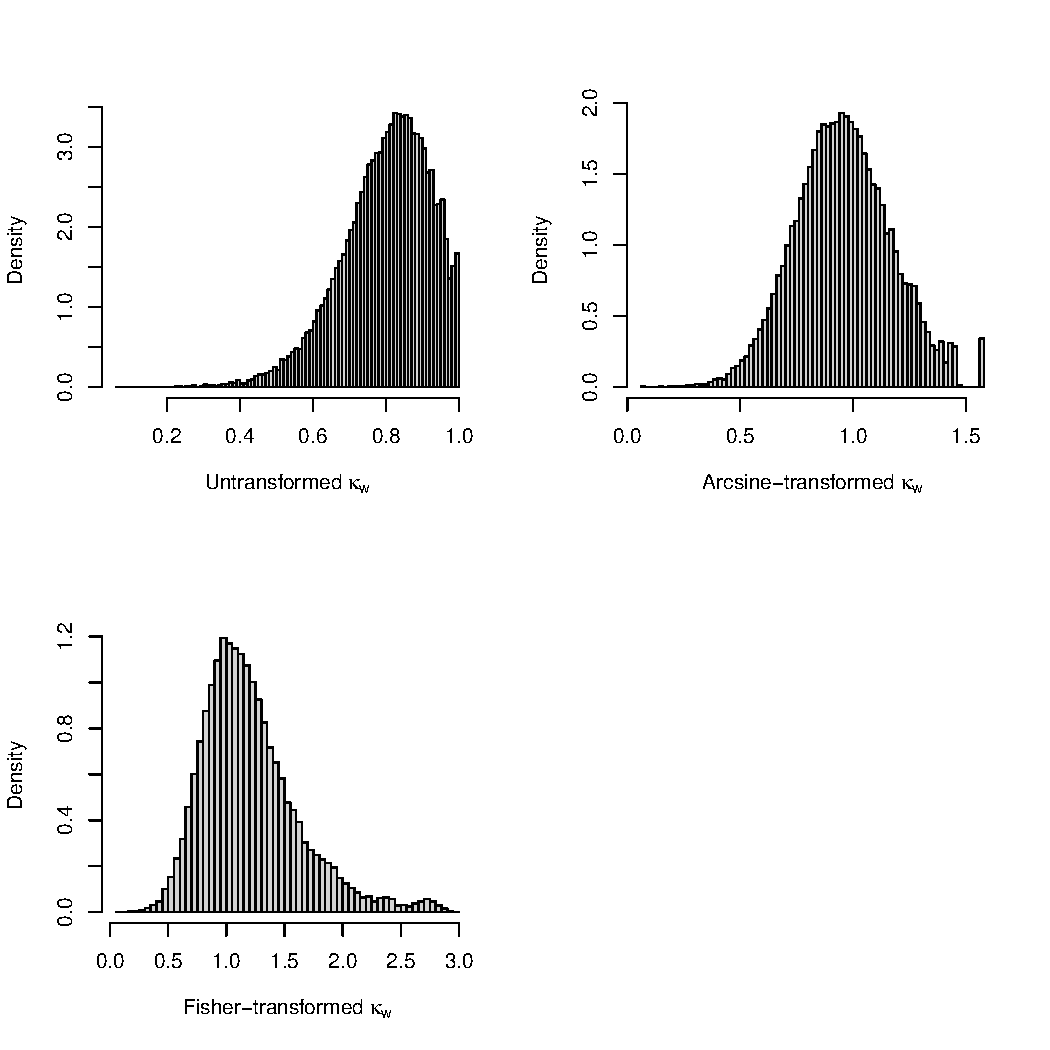
\includegraphics[scale=0.7]{../figures/example_arcsine_fisher_transform}\caption{\label{fig:Fisher transform}Simulated sampling distribution of $\hat{\kappa}_{w}$
for quadratic weights using three transformations, $n=20$, $R=3$.
The simulation setup is described in Example \ref{exa:Fisher transform}.
The arcsine transform makes the sampling distribution closest to the
normal distribution.}
\par\end{centering}
\end{figure}
\end{example}

Calculating the limiting variance of $\arcsin\hat{\kappa}_{d}$ and
$\arcsin\hat{\pi}_{d}$ requires an additional application of the
delta method. We use that $\frac{d}{dx}\arcsin(x)=1/\sqrt{1-x^{2}}$
and $\frac{d}{dx}\artanh(x)=1/(1-x^{2})$. The one-dimensional delta
method states that $\sqrt{n}(\hat{\theta}-\theta)\stackrel{d}{\to}N(0,\sigma^{2})$
implies that $\sqrt{n}(f(\hat{\theta})-f(\theta))\stackrel{d}{\to}N(0,f'(\theta)^{2}\sigma^{2})$.
Hence
\begin{eqnarray}
\sqrt{n}(\arcsin\hat{\kappa}_{d}-\arcsin\kappa_{d}) & \to & N(0,(1-\kappa_{d}^{2})^{-1}\sigma_{\kappa}^{2}),\label{eq:arcsine limit}\\
\sqrt{n}(\artanh\hat{\kappa}_{d}-\artanh\kappa_{d}) & \to & N(0,(1-\kappa_{d}^{2})^{-2}\sigma_{\kappa}^{2}).\label{eq:artanh limit}
\end{eqnarray}
The expressions for $\hat{\pi}_{d}$ can be found by swapping $\kappa_{d}$
for $\pi_{d}$ and $\sigma_{\kappa}^{2}$ for $\sigma_{\pi}^{2}$.

\subsection{Examples}
\begin{example}[\citet{Fleiss1971-to} example (cont.)]
\end{example}

\begin{table}
\caption{\label{tab:fleiss}Confidence intervals for the data of \citet{Fleiss1971-to}
using the arcsine method}

\noindent \begin{centering}
\begin{tabular}{cccccccccccc}
\toprule\textbf{$\boldsymbol{d}$} & \multicolumn{11}{c}{\textbf{Fleiss' kappa}}\tabularnewline
\cmidrule{1-12} & \multicolumn{3}{c}{$g=2$} &  & \multicolumn{3}{c}{$g=3$} &  & \multicolumn{3}{c}{$g=6^{*}$}\tabularnewline
\cmidrule{2-4}\cmidrule{6-8}\cmidrule{10-12} & $\text{CI}_{l}$ & $\text{CI}_{u}$ & \textbf{$\hat{\pi}$} &  & $\text{CI}_{l}$ & $\text{CI}_{u}$ & \textbf{$\hat{\pi}$} &  & $\text{CI}_{l}$ & $\text{CI}_{u}$ & \textbf{$\hat{\pi}$}\tabularnewline
\cmidrule{1-12}$V(d_{0})$ & 0.444 & 0.671 & 0.562 &  & 0.388 & 0.597 & 0.496 &  & 0.366 & 0.597 & 0.486\tabularnewline
Hubert$^{\dagger}$ & 0.444 & 0.671 & 0.562 &  & 0.202 & 0.458 & 0.333 &  & 0.021 & 0.308 & 0.166\tabularnewline
\bottomrule &  &  &  &  &  &  &  &  &  &  & \tabularnewline
\end{tabular}
\par\end{centering}
\vspace{1mm}

{\scriptsize{}$^{*}$This is Hubert's kappa when the Hubert disagreement
is used.}\\
{\scriptsize{}$^{\dagger}$ Hubert disagreement equals the nominal
disagreement $V(d_{0})$ when $g=2$.}{\scriptsize\par}
\end{table}

\citet{Fleiss1971-to}, in the paper introducing what is now called
Fleiss' kappa, discussed an example involving $5$ different kinds
of diagnoses, $n=30$ patients, and $R=6$ psychiatrists. The data
is originally from \citet{Sandifer1968-hz}, but Fleiss removed some
ratings to make the design rectangular. The raters are not the same
for all raters, but it appears plausible to assume that ratings are
exchangeable given the item. The diagnoses are essentially categorical
in nature, hence we will only consider $V(d_{0})$ and Hubert's disagreement
function. The results are shown in Table \ref{tab:fleiss}. We see
that the agreement coefficients agree when $g=2$, as both $V(d_{0})$
and Hubert's disagreement function equals the nominal agreement in
this case. But the coefficients differ substantially as $g$ increases.
This is to be expected, as Hubert's disagreement function measures
consensus while $V(d_{0})$ measures the number of observations different
from the mode.

When $g=R=6$, the difference between Hubert's kappa $(0.166)$ and
$\pi_{V(d_{0})}=0.486$ is substantial, which suggests that a sizeable
number of rating vectors contain at least one rating that disagrees
with the others. Table \ref{tab:counts} summarizes the relevant aspects
of the data. According to the Hubert distance the raters disagree
a lot, as only $5$ items have a distance of $0$ and the rest a distance
of one. On th other hand, $V(d_{0})$ equals $6$ minus the maximal
agreement (i.e., the number of elements distinct from the mode), and
results in much smaller chance-adjusted agreement.

\begin{table}
\caption{\label{tab:counts}Confidence intervals for the data of \citet{Fleiss1971-to}
using the arcsine method}

\begin{centering}
\begin{tabular}{ccccc}
 &  &  &  & \tabularnewline
\toprule Maximal agreement$^{*}$ & $3$ & $4$ & $5$ & $6$\tabularnewline
Count & $8$ & $10$ & $7$ & $5$\tabularnewline
Distance ($V(d_{0})$) & $3$ & $2$ & $1$ & $0$\tabularnewline
Distance (Hubert) & $1$ & $1$ & $1$ & $0$\tabularnewline
\bottomrule &  &  &  & \tabularnewline
\end{tabular} 
\par\end{centering}
\vspace{1mm}

{\scriptsize{}$^{*}$The largest number of raters that agree on the
classification of an item. Both $V(d_{0})$ and Hubert's distance
depend only on this when $g=R$.}{\scriptsize\par}
\end{table}
According to the Hubert distance the raters disagree a lot, as only
$5$ items have a distance of $0$ and the rest a distance of one.
On th other hand, $V(d_{0})$ equals $6$ minus the maximal agreement
(i.e., the number of elements distinct from the mode), and results
in much smaller chance-adjusted agreement.
\begin{example}
\citet{Zapf2016-eu} studied bootstrap intervals for Fleiss' kappa
and Krippendorff's alpha using simulations and a case study. Their
case study concerned histopathological assessment of breast cancer,
and involved ratings done by $R=4$ senior pathologists and $n=50$
breast cancer biopsies. We apply the arcsine method to calculate confidence
intervals and point estimates (Table \ref{tab:Zapf}). We focus on
Cohen's kappa since the same four pathologists rate each cancer biopsy,
but we include a column for Fleiss' kappa when $g=4$ for comparisons
sake. When $g=4$, Cohen's kappa and Fleiss' kappa are as good as
indistinguishable. As can be verified using the code in the supplementary
material, this happens for the other $g$s as well. It is not generally
the case that Fleiss' kappa and Cohen's kappa nearly coincide, but
is likely to happen if the marginal ratings are approximately the
same for all raters, as is the case in this data set. There is a sizable
difference between the disagreement functions, but there is not typically
a big difference when changing $g$s, provided we keep the disagreement
functions constant. It remains to be seen if this common or not. The
exception is Hubert's disagreement function, which decreases by quite
a bit. (As in the \citet{Fleiss1971-to} example, this is expected,
as the Hubert's disagreement function is a consensus measure.) Observe
that the quadratic Fr�chet variance $V(d_{2}^{2})$ does not change
with $g$ at all. The estimators are not exactly the same for the
Cohen type chance agreement, but one can show that the disagreement
at $x$ equals with $g=2+i$ equals $i$ times the disagreement when
$g=2$. This implies that Fleiss' kappa is invariant under $g$.
\end{example}

\begin{table}
\caption{\label{tab:Zapf}Confidence intervals for \citet{Zapf2016-eu} using
the arcsine method}

\noindent \begin{centering}
\begin{tabular}{cccccccccccc}
\toprule$\boldsymbol{d}$ & \multicolumn{7}{c}{\textbf{Cohen's kappa}} &  & \multicolumn{3}{c}{\textbf{Fleiss' kappa}}\tabularnewline
\cmidrule{1-12} & \multicolumn{3}{c}{$g=2$} &  & \multicolumn{3}{c}{$g=4^{\dagger}$} &  & \multicolumn{3}{c}{$g=4$}\tabularnewline
\cmidrule{2-4}\cmidrule{6-8}\cmidrule{10-12} & $\text{CI}_{l}$ & $\text{CI}_{u}$ & \textbf{$\hat{\kappa}$} &  & $\text{CI}_{l}$ & $\text{CI}_{u}$ & \textbf{$\hat{\kappa}$} &  & $\text{CI}_{l}$ & $\text{CI}_{u}$ & \textbf{$\hat{\pi}$}\tabularnewline
\cmidrule{1-12}$V(d_{0})$ & 0.453 & 0.672 & 0.567 &  & 0.471 & 0.699 & 0.591 &  & 0.466 & 0.700 & 0.589\tabularnewline
$V(d_{1})$ & 0.699 & 0.857 & 0.784 &  & 0.711 & 0.870 &  0.798 &  & 0.710 & 0.870 & 0.797\tabularnewline
$V(d_{2}^{2})$ & 0.834 & 0.948 & 0.898 &  & 0.834 & 0.948 &  0.898 &  & 0.834 & 0.948 & 0.898\tabularnewline
Hubert$^{\dagger}$ & 0.453 & 0.672 & 0.567 &  & 0.273 & 0.564 &  0.424 &  & 0.271 & 0.564 & 0.423\tabularnewline
\bottomrule &  &  &  &  &  &  &  &  &  &  & \tabularnewline
\end{tabular}
\par\end{centering}
\vspace{1mm}

{\scriptsize{}$^{\dagger}$ Hubert disagreement equals the nominal
disagreement $V(d_{0})$ when $g=2$.}{\scriptsize\par}
\end{table}


\section{Simulations}

\subsection{Simulation of confidence sets when $g=2$\label{sec:Simulation-of-confidence-k2}}

We include a small simulation study about the performance of confidence
sets using two models.
\begin{enumerate}
\item \textbf{Number of raters} $R$. We use $2,5,20$, corresponding to
a small, medium, and large selection of raters.
\item \textbf{Sample sizes} $n$. We use $n=10,40,100$, corresponding to
small, medium-sized, and large agreement studies. 
\item \textbf{Disagreement functions}. We use the classics: The nominal
disagreement $1[x\neq y]$, quadratic disagreement $(x-y)^{2}$, and
absolute value disagreement $|x-y|$.
\item \textbf{Models.} We simulate from two models. A Perreault--Leigh
model for discrete ratings and a normal model for continuous ratings.
These models are described in more detail below.
\item \textbf{Methods.} We will use three methods for confidence interval
construction: A basic interval without transformations, an arcsine-transformed
interval, and a Fisher-transformed interval. 
\end{enumerate}
We describe our three confidence interval constructions only for Cohen's
kappa, as the intervals using Fleiss' kappa can be found by replacing
every instance $\hat{\kappa}_{d}$ with $\hat{\pi}_{d}$ and $\hat{\sigma}_{\kappa}^{2}$
with $\hat{\sigma}_{\pi}^{2}$. We use two-sided $t$-distribution-based
confidence intervals with nominal level $1-\alpha=0.95$. The\emph{
}basic interval is
\begin{equation}
[\hat{\kappa}_{d}-t_{1-\alpha/2}(n-1)\hat{\sigma}_{\kappa},\hat{\kappa}_{d}+t_{1-\alpha/2}(n-1)\hat{\sigma}_{\kappa}],\label{eq:basic CI}
\end{equation}
where $\hat{\sigma}(\hat{\kappa}_{d})$ is the estimated variance
described in equation (\ref{eq:cohen variance formula}) and $t_{\alpha}(\nu)$
is the $\alpha$-percentile of the $t$-distribution with $\nu$ degrees
of freedom.

In the arcsine interval replaces the basic limits with
\begin{equation}
\sin\left(\arcsin\hat{\kappa}_{d}\pm t_{1-\alpha/2}(n-1)(1-\hat{\kappa}_{d}^{2})^{-1}\hat{\sigma}_{\kappa}^{2}\right),\label{eq:arcsine CI}
\end{equation}
where $(1-\hat{\kappa}_{d}^{2})^{-1}\hat{\sigma}_{\kappa}^{2}$ is
the asymptotic variance of $\arcsin\hat{\kappa}_{d}$ (\ref{eq:arcsine limit}).
The Fisher interval uses the area hyperbolic tangent,
\begin{equation}
\tanh\left(\artanh\hat{\kappa}_{d}\pm t_{1-\alpha/2}(n-1)(1-\hat{\kappa}_{d}^{2})^{-2}\hat{\sigma}_{\kappa}^{2}\right),\label{eq:artanh CI}
\end{equation}
where $(1-\hat{\kappa}_{d}^{2})^{-2}\hat{\sigma}_{\kappa}^{2}$ is
the asymptotic variance of $\artanh\hat{\kappa}_{d}$ (\ref{eq:artanh limit}).

\subsubsection{A Perreault--Leigh model\label{subsec:A-Perreault=002013Leigh-model}}

\citet{Perreault1989-mg} discusses a particular model for ratings
where each rater either knows the correct answer or guesses uniformly
at random. Similar models have been used by \citet{Gwet2008-qk,Maxwell1977-lf},
among others. We assume there are five categories encoded as $C=(-2,-1,0,1,2)$,
and the distribution of the true classification distribution is uniform.
For each item rated, the $j$th rater knows the correct classification
with probability $\sqrt{0.8}$. If not, he guesses, picking a number
from $C$ uniformly at random. Then $\kappa_{d}=\pi_{d}=0.8$ for
all weights and number of raters, as can be verified by following
the arguments of \citet{Perreault1989-mg}. We run each simulation
$N=10,000$ times.

The simulated lengths and coverages for Cohen's kappa are in Table
\ref{tab:Cohen-guessing}. The table for Fleiss' kappa is similar,
and can be found in the appendix, p. \pageref{tab:Fleiss-guessing}.
Two features stand out in Table \ref{tab:Cohen-guessing}. First,
the confidence intervals have almost indistinguishable lengths and
coverages when either $R$ or $n$ is large. Second, the basic interval
has worse coverage than the arcsine and Fisher intervals when $n$
is small, with the Fisher interval having slightly better coverage
than the arcsine interval. However, the better coverage comes at the
expense of greater lengths. In particular, for the absolute value
weight, the coverage of the arcsine interval is greater than the coverage
of the Fisher interval, but its length is shorter.

\begin{table}
\caption{\label{tab:Cohen-guessing}Coverage (first entry) and lengths (second
entry) of confidence intervals: Perreault--Leigh model, Cohen's kappa}

\noindent \begin{centering}
\begin{tabular}{cccccccccccc}
\toprule &  &  & \multicolumn{9}{c}{\textbf{Perreault--Leigh model, Cohen's kappa}}\tabularnewline
\cmidrule{4-12} & \textbf{Method} &  & \multicolumn{3}{c}{$R=2$} & \multicolumn{3}{c}{$R=5$} & \multicolumn{3}{c}{$R=20$}\tabularnewline
 &  & \textbf{$n$} & $10$ & $40$ & $100$ & $10$ & $40$ & $100$ & $10$ & $40$ & $100$\tabularnewline
\midrule \textbf{Weights} &  &  &  &  &  &  &  &  &  &  & \tabularnewline
\cmidrule{4-12}Nominal & Basic &  & 0.81 & \textbf{0.96} & \textbf{0.96} & 0.92 & \textbf{0.95} & \textbf{0.95} & \textbf{0.96} & \textbf{0.95} & \textbf{0.95}\tabularnewline
 &  &  & 0.53 & 0.30 & 0.18 & 0.41 & 0.18 & 0.11 & 0.23 & 0.09 & 0.06\tabularnewline
 & Arcsine &  & \textbf{0.98} & \textbf{0.95} & \textbf{0.95} & \textbf{0.97} & \textbf{0.95} & \textbf{0.95} & \textbf{0.95} & \textbf{0.95} & \textbf{0.95}\tabularnewline
 &  &  & 0.73 & 0.29 & 0.18 & 0.43 & 0.18 & 0.11 & 0.23 & 0.09 & 0.06\tabularnewline
 & Fisher &  & \textbf{0.97} & \textbf{0.96} & \textbf{0.96} & \textbf{0.96} & \textbf{0.95} & \textbf{0.95} & \textbf{0.95} & 0.94 & \textbf{0.95}\tabularnewline
 &  &  & 0.91 & 0.32 & 0.19 & 0.50 & 0.19 & 0.11 & 0.24 & 0.09 & 0.06\tabularnewline
\cmidrule{4-12}Quadratic & Basic &  & 0.65 & 0.87 & 0.92 & 0.84 & 0.93 & \textbf{0.95} & 0.94 & \textbf{0.95} & \textbf{0.95}\tabularnewline
 &  &  & 0.58 & 0.39 & 0.26 & 0.49 & 0.26 & 0.16 & 0.34 & 0.14 & 0.08\tabularnewline
 & Arcsine &  & 0.82 & 0.89 & 0.93 & 0.88 & 0.94 & \textbf{0.95} & 0.94 & \textbf{0.95} & \textbf{0.95}\tabularnewline
 &  &  & 0.78 & 0.39 & 0.25 & 0.55 & 0.26 & 0.16 & 0.34 & 0.14 & 0.08\tabularnewline
 & Fisher &  & \textbf{0.95} & 0.91 & \textbf{0.95} & 0.90 & 0.94 & \textbf{0.95} & 0.93 & \textbf{0.95} & \textbf{0.95}\tabularnewline
 &  &  & 0.94 & 0.44 & 0.27 & 0.65 & 0.27 & 0.16 & 0.37 & 0.14 & 0.08\tabularnewline
\cmidrule{4-12}Absolute value & Basic &  & 0.80 & 0.91 & 0.93 & 0.90 & 0.94 & \textbf{0.95} & \textbf{0.95} & \textbf{0.95} & \textbf{0.95}\tabularnewline
 &  &  & 0.55 & 0.33 & 0.21 & 0.44 & 0.21 & 0.13 & 0.27 & 0.11 & 0.06\tabularnewline
 & Arcsine &  & \textbf{0.98} & 0.94 & \textbf{0.95} & 0.94 & \textbf{0.95} & \textbf{0.95} & \textbf{0.95} & \textbf{0.95} & \textbf{0.95}\tabularnewline
 &  &  & 0.75 & 0.33 & 0.21 & 0.47 & 0.21 & 0.13 & 0.27 & 0.11 & 0.06\tabularnewline
 & Fisher &  & \textbf{0.97} & \textbf{0.95} & \textbf{0.95} & \textbf{0.95} & \textbf{0.95} & \textbf{0.96} & 0.94 & \textbf{0.95} & \textbf{0.95}\tabularnewline
 &  &  & 0.93 & 0.35 & 0.21 & 0.55 & 0.21 & 0.13 & 0.28 & 0.11 & 0.07\tabularnewline
\bottomrule &  &  &  &  &  &  &  &  &  &  & \tabularnewline
\end{tabular}
\par\end{centering}
\vspace{1mm}

{\scriptsize{}Coverages greater than $0.95$ are in bold.}{\scriptsize\par}
\end{table}


\subsubsection{Normal model}

In this study, the rating data is distributed according to the multivariate
normal $N(0,\Sigma)$, where $\Sigma$ is the $R\times R$ correlation
matrix with off-diagonal elements $\Sigma_{j_{1}j_{2}}=\rho$. Recall
that $d_{1}$ denotes the absolute value disagreement and $d_{2}^{2}$
the quadratic disagreement. The true values are $\kappa_{d_{2}}=\pi_{d_{2}^{2}}=\rho$
and $\kappa_{d_{1}}=\pi_{d_{1}}=1-\sqrt{1-\rho}$. See the appendix
(p. \pageref{subsec:true values}) for details on the computation
of these true value. We use $\rho=0.7$, hence $\kappa_{d_{2}^{2}}=0.7$
and $\kappa_{\textrm{\ensuremath{d_{1}}}}=0.45$. Note that the nominal
weight will not work for this continuous data, hence we simulate using
only the quadratic and absolute value weights. We run each simulation
$N=1,000$ times\footnote{We use fewer simulations ($1,000$) than in the previous simulation
($10,000$) since estimation is far more computationally expensive
when dealing with continuous data, as it does not allow for binning. }. We note that agreement coefficients are frequently called concordance
coefficients when dealing with continuous data. Lin's concordance
coefficient \citep{Lin1989-kf} is a prominent example. 

The simulated lengths and coverages for Cohen's kappa are in Table
\ref{tab:cohen-normal}. The table for Fleiss' kappa is similar, and
can be found in the appendix (p. \pageref{tab:Fleiss-normal}). From
the table below, we see that there is barely any difference between
the three confidence interval constructions. Taken together with the
results for the Perreault--Leigh model, where the basic interval
performs worse than the other two, we would recommend the usage of
either the arcsine or Fisher interval.
\noindent \begin{center}
\begin{table}
\noindent \begin{centering}
\caption{\label{tab:cohen-normal}Coverage (first entry) and lengths (second
entry) of confidence intervals: Normal model, Cohen's kappa}
\begin{tabular}{cccccccccccc}
\toprule & \multicolumn{11}{c}{\textbf{Cohen's kappa: Normal model}}\tabularnewline
\cmidrule{4-12} & \textbf{Method} &  & \multicolumn{3}{c}{$R=2$} & \multicolumn{3}{c}{$R=5$} & \multicolumn{3}{c}{$R=20$}\tabularnewline
 &  & \textbf{$n$} & $10$ & $40$ & $100$ & $10$ & $40$ & $100$ & $10$ & $40$ & $100$\tabularnewline
\midrule \textbf{Weights} &  &  &  &  &  &  &  &  &  &  & \tabularnewline
\cmidrule{4-12}Quadratic & Basic &  & 0.88 & 0.92 & \textbf{0.95} & 0.91 & \textbf{0.95} & 0.94 & 0.88 & 0.93 & \textbf{0.95}\tabularnewline
 &  &  & 0.66 & 0.32 & 0.20 & 0.50 & 0.23 & 0.14 & 0.43 & 0.20 & 0.12\tabularnewline
 & Arcsine &  & 0.88 & 0.93 & \textbf{0.95} & 0.90 & \textbf{0.95} & 0.94 & 0.87 & 0.92 & 0.94\tabularnewline
 &  &  & 0.67 & 0.32 & 0.20 & 0.49 & 0.23 & 0.14 & 0.42 & 0.20 & 0.12\tabularnewline
 & Fisher &  & 0.90 & 0.94 & 0.94 & 0.88 & 0.94 & 0.94 & 0.86 & 0.92 & 0.94\tabularnewline
 &  &  & 0.70 & 0.33 & 0.20 & 0.51 & 0.23 & 0.14 & 0.43 & 0.20 & 0.12\tabularnewline
\cmidrule{4-12}Absolute value & Basic &  & 0.92 & 0.94 & 0.94 & 0.92 & 0.93 & \textbf{0.95} & 0.87 & 0.94 & 0.94\tabularnewline
 &  &  & 0.67 & 0.31 & 0.19 & 0.46 & 0.21 & 0.13 & 0.38 & 0.18 & 0.11\tabularnewline
 & Arcsine &  & 0.93 & 0.94 & 0.94 & 0.92 & 0.93 & \textbf{0.95} & 0.87 & 0.94 & 0.94\tabularnewline
 &  &  & 0.65 & 0.31 & 0.19 & 0.45 & 0.21 & 0.13 & 0.38 & 0.18 & 0.11\tabularnewline
 & Fisher &  & 0.93 & 0.94 & \textbf{0.95} & 0.92 & 0.93 & \textbf{0.95} & 0.86 & 0.94 & 0.94\tabularnewline
 &  &  & 0.65 & 0.31 & 0.19 & 0.45 & 0.21 & 0.13 & 0.38 & 0.18 & 0.11\tabularnewline
\bottomrule &  &  &  &  &  &  &  &  &  &  & \tabularnewline
\end{tabular}
\par\end{centering}
\vspace{1mm}

{\scriptsize{}Coverages greater than $0.95$ are in bold.}{\scriptsize\par}
\end{table}
\par\end{center}

\subsection{Simulation of confidence sets when $g\protect\neq2$\label{sec:Simulation-of-confidence-kj}}

Table \ref{tab:Cohen-guessing-multi} contains simulations from the
Perreault--Leigh model (p. \pageref{subsec:A-Perreault=002013Leigh-model})
with $N=1000$ repetitions and $R=5$ raters using the Fr�chet variances
$V(d_{0})$, $V(d_{1})$, $V(d_{2}^{2})$, and Hubert's disagreement
function. To save space, we drop the basic confidence interval in
the simulation. As before, we show the results only for the Cohen-type
disagreement, with the Fleiss-type disagreement relegated to the appendix
(p. \pageref{tab:fleiss-guessing-multi}). The methods have virtually
indistinguishable properties, with very similar coverages and lengths
across the board. All coverages are decent, with the exception of
the quadratic Fr�chet variance with small $n$, where the coverage
drops into the high 80s.

\begin{table}
\caption{\label{tab:Cohen-guessing-multi}Coverage (first entry) and lengths
(second entry) of confidence intervals: Perreault--Leigh model, Cohen's
kappa}

\noindent \begin{centering}
\begin{tabular}{cccccccccccc}
\toprule &  &  & \multicolumn{9}{c}{\textbf{Perreault--Leigh model, Cohen's kappa}}\tabularnewline
\cmidrule{4-12} & \textbf{Method} &  & \multicolumn{3}{c}{$g=3$} & \multicolumn{3}{c}{$g=4$} & \multicolumn{3}{c}{$g=5$}\tabularnewline
 &  & \textbf{$n$} & $10$ & $40$ & $100$ & $10$ & $40$ & $100$ & $10$ & $40$ & $100$\tabularnewline
\midrule \textbf{Weights} &  &  &  &  &  &  &  &  &  &  & \tabularnewline
\cmidrule{4-12}$V(d_{0})$ & Arcsine &  & \textbf{0.98} & \textbf{0.96} & 0.94 & \textbf{0.97} & \textbf{0.95} & 0.94 & \textbf{0.98} & 0.93 & 0.93\tabularnewline
 &  &  & 0.41 & 0.16 & 0.10 & 0.39 & 0.16 & 0.10 & 0.38 & 0.15 & 0.09\tabularnewline
 & Fisher &  & \textbf{0.96} & \textbf{0.96} & 0.94 & \textbf{0.96} & \textbf{0.96} & 0.94 & \textbf{0.96} & 0.94 & 0.94\tabularnewline
 &  &  & 0.46 & 0.17 & 0.10 & 0.44 & 0.16 & 0.10 & 0.42 & 0.15 & 0.09\tabularnewline
\cmidrule{4-12}$V(d_{1})$ & Arcsine &  & 0.94 & 0.94 & \textbf{0.95} & 0.94 & 0.94 & 0.94 & 0.94 & \textbf{0.95} & \textbf{0.95}\tabularnewline
 &  &  & 0.49 & 0.21 & 0.13 & 0.45 & 0.19 & 0.11 & 0.44 & 0.19 & 0.11\tabularnewline
 & Fisher &  & \textbf{0.96} & 0.94 & \textbf{0.95} & \textbf{0.95} & \textbf{0.95} & \textbf{0.95} & \textbf{0.96} & \textbf{0.95} & \textbf{0.95}\tabularnewline
 &  &  & 0.55 & 0.21 & 0.13 & 0.51 & 0.19 & 0.12 & 0.51 & 0.19 & 0.12\tabularnewline
\cmidrule{4-12}$V(d_{2}^{2})$ & Arcsine &  & 0.90 & 0.94 & \textbf{0.96} & 0.88 & 0.94 & 0.94 & 0.88 & 0.93 & 0.94\tabularnewline
 &  &  & 0.56 & 0.25 & 0.16 & 0.56 & 0.26 & 0.16 & 0.57 & 0.25 & 0.16\tabularnewline
 & Fisher &  & 0.92 & 0.94 & \textbf{0.96} & 0.91 & \textbf{0.95} & \textbf{0.95} & 0.89 & 0.94 & \textbf{0.95}\tabularnewline
 &  &  & 0.65 & 0.27 & 0.16 & 0.65 & 0.27 & 0.16 & 0.66 & 0.27 & 0.16\tabularnewline
\cmidrule{4-12}Hubert & Arcsine &  & \textbf{0.98} & \textbf{0.95} & \textbf{0.96} & \textbf{0.98} & \textbf{0.95} & \textbf{0.96} & \textbf{0.98} & \textbf{0.95} & \textbf{0.95}\tabularnewline
 &  &  & 0.52 & 0.22 & 0.13 & 0.62 & 0.26 & 0.16 & 0.71 & 0.31 & 0.19\tabularnewline
 & Fisher &  & \textbf{0.97} & \textbf{0.96} & \textbf{0.96} & \textbf{0.97} & \textbf{0.96} & \textbf{0.96} & \textbf{0.98} & \textbf{0.96} & 0.94\tabularnewline
 &  &  & 0.57 & 0.22 & 0.13 & 0.67 & 0.27 & 0.16 & 0.77 & 0.31 & 0.19\tabularnewline
\bottomrule &  &  &  &  &  &  &  &  &  &  & \tabularnewline
\end{tabular}
\par\end{centering}
\vspace{1mm}

{\scriptsize{}Coverages greater than $0.95$ are in bold.}{\scriptsize\par}
\end{table}


\section{Concluding remarks}

When choosing an agreement coefficient one has to carefully think
through exactly what one wishes to measure. The Fr�chet variances
are attractive due to their interpretation. You measure how much do
the raters disagree with the (generalized) mean rater, and then adjust
for chance. In the case of nominal data, we measure disagreement with
the modal rater. When dealing with numerical data, we may measure
disagreement with the median rater (using the absolute value distance),
or the mean rater (using the quadratic distance), or use any other
Fr�chet variance defined on numeric data.

When dealing with nominal data, we believe that using the Fr�chet
variance that measures the distance from the mode is a reasonable
choice. But other options are certainly possible, even when dealing
with $g$-wise agreement measures. For instance, one could use the
entropy instead, with distance measure $d(x_{1},x_{2},\ldots,x_{g})=-\sum_{i=1}^{g}\frac{\#i}{g}\log\frac{\#i}{g},$where
$\#i$ counts the number of elements in $(x_{1},x_{2},\ldots,x_{g})$
classified as $i$. The topic of how to choose reasonable distance
measures for $g$-wise agreement studies has not been thoroughly studied,
and there might be options preferable to the Fr�chet variances that
have not yet been found.

We have only covered rectangular design, where every item is rated
by the same number of raters. It is quite easy to generalize the definitions
of $\kappa_{d}$ and $\pi_{d}$ to non-rectangular designs, as we
have done in the appendix, p. \pageref{subsec:Expanding-the-definitions}.
But inference appears to be quite difficult, probably requiring additional
assumptions for the case of non-exchangeable ratings.

The confidence intervals based on the arcsine and Fisher transforms
perform better than the basic, untransformed interval. It is unclear
which one of these intervals to prefer, but it barely matters when
the sample size is sufficiently large. It might be possible to improve
all of these intervals. Small-sample corrections to the variance appears
feasible, with potential openings in the in the application of the
delta rule and in the calculation of $\Sigma$ of Lemma \pageref{lem:limit lemma}.
We have used the arcsine and Fisher transforms to improve approximate
normality of $\hat{\kappa}_{d}$ and $\hat{\pi}_{d}$, but this choice
is semi-arbitrary. Better variance-stabilizing transformations might
be found by inspecting the formula for the variances of $\hat{\kappa}_{d}$
and $\hat{\pi}_{d}$ in Proposition \ref{prop:The-asymptotic-variances}.
The confidence intervals used in the simulation are only known to
be first-order accurate. To make second-order accurate confidence
intervals, it would be possible to use the explicit formula for the
variances to construct studentized confidence intervals, i.e., bootstrap-$t$
intervals \citep{Efron1987-ov}, which are second-order accurate. 

None of these approaches are guaranteed to help when $n$ is small,
especially when dealing with categorical data, as the sampling distributions
of $\hat{\kappa}_{d}$ and $\hat{\pi}_{d}$ are discrete and highly
irregular. For example, consider the sample distribution of the Perreault--Leigh
model (section \ref{sec:Simulation-of-confidence-k2}) when $n=20$
and $R=20$, displayed in Figure \ref{fig:irregular}. (We omit a
dominating spike at $1$.) As there are $C=5<\infty$ categories,
there is a finite number of possible values for $\hat{\kappa}_{d}$
to take, which is strongly reflected in the plots, especially for
the nominal weight. 

\begin{figure}
\noindent \centering{}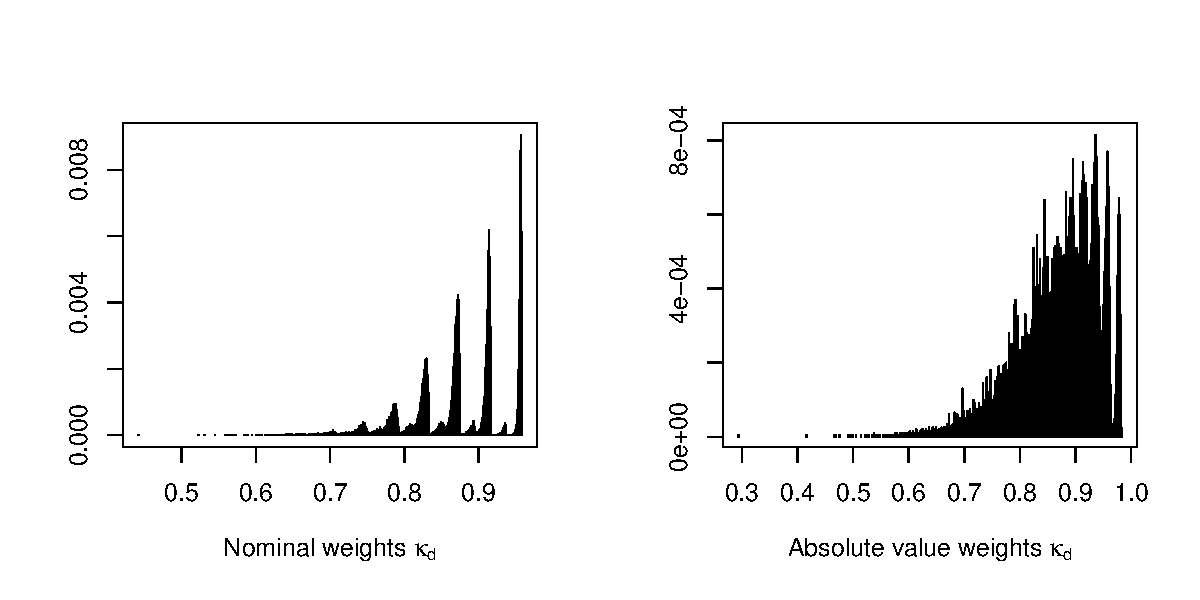
\includegraphics[scale=0.7]{../figures/example_irregular}\caption{\label{fig:irregular}Sample distribution of $\hat{\kappa}_{d}$ for
nominal (left) and absolute value (right) weights. Both plots omit
a dominating spike at $1$. Here $n=20$ and $j=5$, and we use the
Perreault--Leigh model (same parameters as in section \ref{sec:Simulation-of-confidence-k2})
to simulate the data. There were $2573$ unique values for the nominal
weight and $8790$ unique values for the absolute value weight after
$N=200,000$ simulations. }
\end{figure}

The superior performance of methods such as the bootstrap-$t$ depend
on the quantity $\frac{\hat{\theta}-\theta}{\se}$ being approximately
pivotal, i.e., approximately the same for all parameters, possibly
after applying a transformation. Judging from the plots above, there
is no such transformation.

\bibliographystyle{apacite}
\bibliography{kappa-sd}


\section*{Appendix}

\subsection*{Agreement vs disagreement \label{subsec:Agreement-vs-disagreement}}

Agreement weighting functions are frequently standardized to guarantee
that $w(x_{1},x_{2})\geq0$, e.g., $w(x_{1},x_{2})=1-|x_{1}-x_{2}|/\max(|x_{1}-x_{2}|)$
for the absolute value weights. The standardization is not necessary,
as they do not change the value of $\kappa_{d}$ and $\pi_{d}$ when
it is possible (i.e., when $\max(|x_{1}-x_{2}|)<\infty$), and is
undefined otherwise. We choose not use this operation, as it does
not change the value of the agreement coefficients in this paper,
and is impossible to do when the range of $x_{1},x_{2}$ is unbounded. 

\subsection*{Proof of equivalence between $V(d_{p})(\boldsymbol{x}_{1},\boldsymbol{x}_{2})$
and $||\boldsymbol{x}_{1}-\boldsymbol{x}_{2}||$\label{subsec:Proof-of-equivalence}}
\begin{proof}
We will show that
\[
V(d_{p})[\boldsymbol{x}_{1},\boldsymbol{x}_{2}]=\frac{1}{2}||\boldsymbol{x}_{1}-\boldsymbol{x}_{2}||_{p},\quad V(d_{p}^{p})[\boldsymbol{x}_{1},\boldsymbol{x}_{2}]=\frac{1}{2^{p}}||\boldsymbol{x}_{1}-\boldsymbol{x}_{2}||_{p}^{p}.
\]
First, consider the case when $p\geq1$. Using translation invariance
and homogeneity of the norm,
\begin{eqnarray*}
 &  & ||x_{1}-\mu||_{p}+||x_{2}-\mu||_{p},\\
 & = & ||x_{1}-\frac{x_{1}+x_{2}}{2}-\mu+\frac{x_{1}+x_{2}}{2}||_{p}+||x_{2}-\frac{x_{1}+x_{2}}{2}-\mu+\frac{x_{1}+x_{2}}{2}||_{p},\\
 & = & ||\frac{x_{1}-x_{2}}{2}-\nu||_{p}+||-\frac{x_{1}-x_{2}}{2}-\nu||_{p},\\
 & = & ||a-\nu||_{p}+||a+\nu||_{p},
\end{eqnarray*}
where $a=\frac{x_{1}-x_{2}}{2}$ and $\nu=\mu-\frac{x_{1}+x_{2}}{2}$.

Observe that
\[
\argmin_{\nu}||a+\nu||_{p}+||a-\nu||_{p}=0,\quad\text{for all }a
\]
implies $\mu=\frac{x_{1}+x_{2}}{2}$. 

By the Minkowski inequality,
\[
2^{p}||a||^{p}=||a+\nu+a-\nu||^{p}\leq(||a-\nu||+||a+\nu||)^{p}.
\]
This is an equality if $||a-\nu||=||a+\nu||=||a||$, i.e., when $\nu=0,$
as the left side equals $(||a-\mu||+||a+\mu||)^{p}=2^{p}||a||^{p}$.
Now it's easy to verify that $V(d_{p})$ and $V(d_{p}^{p})$ have
the claimed form; just substitute the value $\mu=\frac{x_{1}+x_{2}}{2}$
into the formula for the Fr�chet variance, $\frac{1}{2}(||x_{1}-\mu||_{p}+||x_{2}-\mu||_{p})$. 

When $0<p<1$, the function $\mu\mapsto||x_{1}-\mu||_{p}+||x_{2}-\mu||_{p}$
is stepwise concave on $[-\infty,x_{1}]$,$[x_{1},x_{2}]$, and $[x_{2},\infty)$,
hence its minimum is either $x_{1},x_{2}$, or both. It's clear that
both $x_{1}$ and $x_{2}$ maps to $||x_{1}-x_{2}||_{p}$, hence both
are Fr�chet means. The case $p=0$ is obvious and omitted.
\end{proof}

\subsection*{True values in the normal simulation\label{subsec:true values}}

We give a brief explanation why the true values of $\kappa_{d}$ and
$\pi_{d}$ are $0.8$ for the quadratic weights and $1-\sqrt{0.2}$
for the absolute value weights. 

First notice that, since the marginals of $X_{j_{1}}$ and $X_{j_{2}}$
are equal for all $j_{1},j_{2}$, we have that $\kappa_{d}=\pi_{d}$.
Moreover, we can ignore the number of raters, since the pairwise distribution
do not depend on them. Then, from standard theory about the multivariate
and folded normal, we find that
\[
E(|X_{j_{1}}-X_{j_{2}}|)=2\sqrt{\frac{1-\rho}{\pi}},\quad E(|X_{j_{1}}-X_{j_{2}}|^{2})=2(1-\rho).
\]
Let $X'_{j_{1}}$be a copy of $X_{j_{1}}$ that is independent of
$X_{j_{2}}$. Then $E(|X'_{j_{1}}-X_{j_{2}}|)=2/\sqrt{\pi}$ and $E(|X'_{j_{1}}-X_{j_{2}}|^{2})=2$.
Now rewrite the kappas using disagreement instead of agreement. Use
the fact that $(p_{wa}-p_{fa})/(1-p_{fa})=1-d_{wa}/d_{fa}$, where
$d_{wa}=1-E(w(X_{j_{1}},X_{j_{2}}))$ and $d_{fa}=1-E(w(X'_{j_{1}},X_{j_{2}}))$,
where $X'_{j_{1}}$is a copy of $X_{j_{1}}$ that is independent of
$X_{j_{2}}$.

Thus $\kappa_{d}=\pi_{d}=1-E(|X_{j_{1}}-X_{j_{2}}|)/E(|X'_{j_{1}}-X_{j_{2}}|^{2})=1-\sqrt{1-\rho}$
for the absolute value weights and $1-E(|X_{j_{1}}-X_{j_{2}}|^{2})/E(|X'_{j_{1}}-X_{j_{2}}|^{2})=\rho$
for the quadratic weights.

\subsection*{Variance of $U$-statistics\label{subsec:Variance-of--statistics}}

Let $U_{n}^{1}$ and $U_{n}^{2}$ be two $U$-statistics of $n$ observations
with symmetric kernel functions $\psi_{1}$, $\psi_{2}$ of dimension
$k_{1}$ and $k_{2}$. Define

\begin{eqnarray*}
\sigma_{cc}^{2} & = & \Cov(E[\psi_{1}(X_{1},\ldots,X_{k_{1}})\mid X_{1},\ldots,X_{c})],E[\psi_{2}(X_{1},\ldots,X_{k_{2}})\mid X_{1},\ldots,X_{c})]).
\end{eqnarray*}

\begin{prop}
The exact covariance of $U_{1}^{n}$ and $U_{2}^{n}$ is
\[
\Cov(U_{1}^{n},U_{2}^{n})=\binom{n}{k_{1}}^{-1}\sum_{c=1}^{k_{1}}\binom{k_{2}}{c}\binom{n-k_{2}}{k_{1}-c}\sigma_{cc}^{2}.
\]
If $k_{1}$ and $k_{2}$ are fixed, its asymptotic variance is $n\Cov(U_{1}^{n},U_{2}^{n})\to k_{1}k_{2}\sigma_{11}^{2}$. 
\end{prop}

\begin{proof}
See \citep[Theorem 2, p. 17]{Lee2019-xm} and \citep[Theorem 2, p. 76]{Lee2019-xm}
for a proof.
\end{proof}

\subsection*{Expanding the definitions\label{subsec:Expanding-the-definitions}}

Here is sketch of how we could expand the definitions in Section \ref{sec:Pairwise-kappa-like-statistics}
to encompass more complicated scenarios. We restrict ourselves to
$g=2$, but the analysis can be expanded to arbitrary $g$. Suppose
that any infinite number of raters $R$ is possible, the raters are
not exchangeable, and that not every item is rated by every rater. 

Let $X$ denote a rating, $J$ be a raters, and $I$ be the items
rated. Suppose we sample pairs $(X_{1},J_{1},I_{1}),(X_{2},J_{2},I_{2})$
independently from the same distribution $F$. Then we may define
\begin{eqnarray}
D_{d} & = & E[d(X_{1},X_{2})\mid I_{1}=I_{2},J_{1}\neq J_{2}],\label{eq:new_definitions}\\
C_{d} & = & E[d(X_{1},X_{2})\mid J_{1}\neq J_{2}],\nonumber \\
F_{d} & = & E[d(X_{1},X_{2})].\nonumber 
\end{eqnarray}
These quantities have natural sample analogues, e.g., 
\[
\hat{D}_{d}=N^{-1}\sum_{i=1}^{n}\sum_{j_{1}\neq j_{2}}d(x_{ij_{1}},x_{ij_{2}}),
\]
where $N$ is the total number of paired observations and the rater
indices run over the raters who observed at the $i$th observation
$x$. Population and sample definitions of Cohen's kappa and Fleiss'
kappa follow as laid out in the main text, e.g. $\kappa_{d}=1-D_{d}/C_{d}$.

\subsubsection*{Krippendorff's alpha}

Now suppose that the ratings can take on only a finite number $C$
distinct values. Define $o_{ck}$ as the number of times a pair of
raters has classified an item into $c$ and $k$, i.e., 
\[
o_{ck}=\sum_{i=1}^{n}\sum_{j_{1}\neq j_{2}}1[x_{ij_{1}}=c,x_{ij_{2}}=k].
\]
Then $N=\sum_{c,k}o_{ck}$ and $\hat{D}_{d}=N^{-1}\sum_{c,k}o_{ck}d(c,k).$
Moreover, define $n_{c}$ as the number of items classified as $c$.
Then $n_{c}=\sum_{k}o_{ck}$, $\sum_{c}n_{c}=N$, and $\sum_{c,k}n_{c}n_{k}d(c,k)=N^{2}\hat{F}_{d}.$
\begin{prop}
\label{prop:krippendorfff}Using the definitions above, $\hat{\alpha}_{d}=\hat{\pi}_{d}+\frac{1}{N}(1-\hat{\pi}_{d})$.
Since there are $N=2Rn$ rating pairs in the rectangular setup used
in Section \ref{sec:Pairwise-kappa-like-statistics}, $\hat{\alpha}_{w}=\hat{\pi}_{w}+\frac{1}{2Rn}(1-\hat{\pi}_{w})$
in that case.
\end{prop}

\begin{proof}
The definition of $\hat{\alpha}_{w}$ can be found on \citet[p .235]{Krippendorff2018-qk},
\[
\hat{\alpha}_{w}=1-(N-1)\frac{\sum_{c\neq k}o_{ck}d(c,k)}{\sum_{c\neq k}n_{c}n_{k}d(c,k)}.
\]
From the definitions above, and the fact that $d(c,k)=0$ when $c=k$,
we find that
\[
\sum_{c\neq k}o_{ck}d(c,k)=\sum_{c,k}o_{ck}d(c,k)=N\hat{D}_{d}.
\]
In the same way,
\[
\sum_{c\neq k}n_{c}n_{k}d(c,k)=\sum_{c,k}n_{c}n_{k}d(c,k)=N^{2}\hat{F}_{d}.
\]
Thus
\[
\hat{\alpha}_{d}=1-\frac{(N-1)}{N}\frac{\hat{D}_{d}}{\hat{F}_{d}}=1-\frac{\hat{D}_{d}}{\hat{F}_{d}}+\frac{1}{N}\frac{\hat{D}_{d}}{\hat{F}_{d}},
\]
and using that $\hat{\pi}_{d}=1-\frac{\hat{D}_{d}}{\hat{F}_{d}}$,
we're done.
\end{proof}

\subsection*{Simulation of Fleiss' kappa\label{subsec:fleiss simulations}}

Here are the results of the simulation study in \ref{sec:Simulation-of-confidence-k2}
for Fleiss' kappa.

\begin{table}
\caption{\label{tab:Fleiss-guessing}Coverage (first entry) and lengths (second
entry) of confidence intervals: Perreault--Leigh model, Fleiss' kappa}

\noindent \centering{}%
\begin{tabular}{cccccccccccc}
\toprule &  &  & \multicolumn{9}{c}{\textbf{Fleiss' kappa: Perreault--Leigh model}}\tabularnewline
\cmidrule{4-12} & \textbf{Method} &  & \multicolumn{3}{c}{$R=2$} & \multicolumn{3}{c}{$R=5$} & \multicolumn{3}{c}{$R=20$}\tabularnewline
 &  & \textbf{$n$} & $10$ & $40$ & $100$ & $10$ & $40$ & $100$ & $10$ & $40$ & $100$\tabularnewline
\midrule \textbf{Weights} &  &  &  &  &  &  &  &  &  &  & \tabularnewline
\cmidrule{4-12}Nominal & Basic &  & 0.82 & 0.95 & 0.95 & 0.93 & 0.95 & 0.95 & 0.96 & 0.95 & 0.96\tabularnewline
 &  &  & 0.55 & 0.30 & 0.18 & 0.41 & 0.18 & 0.11 & 0.23 & 0.09 & 0.06\tabularnewline
 & Arcsine &  & 0.98 & 0.94 & 0.94 & 0.98 & 0.95 & 0.95 & 0.95 & 0.95 & 0.95\tabularnewline
 &  &  & 0.76 & 0.30 & 0.18 & 0.44 & 0.18 & 0.11 & 0.23 & 0.09 & 0.06\tabularnewline
 & Fisher &  & 0.97 & 0.96 & 0.96 & 0.96 & 0.96 & 0.95 & 0.95 & 0.94 & 0.95\tabularnewline
 &  &  & 0.95 & 0.32 & 0.19 & 0.51 & 0.19 & 0.11 & 0.24 & 0.09 & 0.06\tabularnewline
\cmidrule{4-12}Quadratic & Basic &  & 0.65 & 0.86 & 0.92 & 0.85 & 0.93 & 0.94 & 0.94 & 0.95 & 0.95\tabularnewline
 &  &  & 0.60 & 0.39 & 0.26 & 0.50 & 0.26 & 0.16 & 0.34 & 0.14 & 0.08\tabularnewline
 & Arcsine &  & 0.83 & 0.89 & 0.93 & 0.89 & 0.94 & 0.94 & 0.94 & 0.95 & 0.95\tabularnewline
 &  &  & 0.82 & 0.39 & 0.25 & 0.56 & 0.26 & 0.16 & 0.34 & 0.14 & 0.08\tabularnewline
 & Fisher &  & 0.96 & 0.91 & 0.94 & 0.91 & 0.94 & 0.95 & 0.93 & 0.95 & 0.95\tabularnewline
 &  &  & 0.98 & 0.44 & 0.27 & 0.67 & 0.27 & 0.16 & 0.37 & 0.14 & 0.08\tabularnewline
\cmidrule{4-12}Absolute value & Basic &  & 0.81 & 0.92 & 0.94 & 0.91 & 0.95 & 0.95 & 0.95 & 0.95 & 0.95\tabularnewline
 &  &  & 0.57 & 0.33 & 0.21 & 0.44 & 0.21 & 0.13 & 0.27 & 0.11 & 0.06\tabularnewline
 & Arcsine &  & 0.99 & 0.93 & 0.95 & 0.94 & 0.95 & 0.95 & 0.95 & 0.95 & 0.95\tabularnewline
 &  &  & 0.79 & 0.33 & 0.21 & 0.48 & 0.21 & 0.13 & 0.27 & 0.11 & 0.06\tabularnewline
 & Fisher &  & 0.97 & 0.95 & 0.95 & 0.96 & 0.95 & 0.95 & 0.94 & 0.95 & 0.95\tabularnewline
 &  &  & 0.97 & 0.36 & 0.21 & 0.56 & 0.21 & 0.13 & 0.28 & 0.11 & 0.07\tabularnewline
\bottomrule &  &  &  &  &  &  &  &  &  &  & \tabularnewline
\end{tabular}
\end{table}

\noindent \begin{center}
\begin{table}
\noindent \centering{}\caption{\label{tab:Fleiss-normal}Coverage (first entry) and lengths (second
entry) of confidence intervals: Normal model, Fleiss' kappa}
\begin{tabular}{cccccccccccc}
\toprule & \multicolumn{11}{c}{\textbf{Fleiss' kappa: Normal model}}\tabularnewline
\cmidrule{4-12} & \textbf{Method} &  & \multicolumn{3}{c}{$R=2$} & \multicolumn{3}{c}{$R=5$} & \multicolumn{3}{c}{$R=20$}\tabularnewline
 &  & \textbf{$n$} & $10$ & $40$ & $100$ & $10$ & $40$ & $100$ & $10$ & $40$ & $100$\tabularnewline
\midrule \textbf{Weights} &  &  &  &  &  &  &  &  &  &  & \tabularnewline
Quadratic & Basic &  & 0.89 & 0.93 & 0.95 & 0.90 & 0.95 & 0.94 & 0.90 & 0.93 & 0.95\tabularnewline
 &  &  & 0.70 & 0.33 & 0.20 & 0.50 & 0.23 & 0.14 & 0.42 & 0.20 & 0.12\tabularnewline
 & Arcsine &  & 0.90 & 0.93 & 0.95 & 0.90 & 0.95 & 0.94 & 0.90 & 0.92 & 0.94\tabularnewline
 &  &  & 0.71 & 0.32 & 0.20 & 0.49 & 0.23 & 0.14 & 0.42 & 0.20 & 0.12\tabularnewline
 & Fisher &  & 0.92 & 0.93 & 0.95 & 0.89 & 0.94 & 0.94 & 0.88 & 0.92 & 0.94\tabularnewline
 &  &  & 0.74 & 0.33 & 0.20 & 0.51 & 0.23 & 0.14 & 0.43 & 0.20 & 0.12\tabularnewline
Absolute value & Basic &  & 0.92 & 0.95 & 0.95 & 0.91 & 0.96 & 0.93 & 0.90 & 0.93 & 0.93\tabularnewline
 &  &  & 0.71 & 0.32 & 0.20 & 0.47 & 0.21 & 0.13 & 0.39 & 0.18 & 0.11\tabularnewline
 & Arcsine &  & 0.92 & 0.95 & 0.95 & 0.90 & 0.95 & 0.92 & 0.89 & 0.93 & 0.93\tabularnewline
 &  &  & 0.69 & 0.32 & 0.20 & 0.46 & 0.21 & 0.13 & 0.39 & 0.18 & 0.11\tabularnewline
 & Fisher &  & 0.92 & 0.95 & 0.95 & 0.90 & 0.95 & 0.93 & 0.89 & 0.93 & 0.93\tabularnewline
 &  &  & 0.68 & 0.32 & 0.20 & 0.46 & 0.21 & 0.13 & 0.39 & 0.18 & 0.11\tabularnewline
\bottomrule &  &  &  &  &  &  &  &  &  &  & \tabularnewline
\end{tabular}
\end{table}
\begin{table}
\caption{\label{tab:fleiss-guessing-multi}Coverage (first entry) and lengths
(second entry) of confidence intervals: Perreault--Leigh model, Fleiss'
kappa ($R=5$)}

\noindent \centering{}%
\begin{tabular}{cccccccccccc}
\toprule &  &  & \multicolumn{9}{c}{\textbf{Perreault--Leigh model, Fleiss' kappa}}\tabularnewline
\cmidrule{4-12} & \textbf{Method} &  & \multicolumn{3}{c}{$g=3$} & \multicolumn{3}{c}{$g=4$} & \multicolumn{3}{c}{$g=5$}\tabularnewline
 &  & \textbf{$n$} & $10$ & $40$ & $100$ & $10$ & $40$ & $100$ & $10$ & $40$ & $100$\tabularnewline
\midrule \textbf{Weights} &  &  &  &  &  &  &  &  &  &  & \tabularnewline
\cmidrule{4-12}$V(d_{0})$ & Arcsine &  & 0.97 & 0.94 & 0.96 & 0.98 & 0.95 & 0.95 & 0.98 & 0.95 & 0.94\tabularnewline
 &  &  & 0.41 & 0.16 & 0.10 & 0.39 & 0.16 & 0.10 & 0.38 & 0.15 & 0.09\tabularnewline
 & Fisher &  & 0.96 & 0.94 & 0.96 & 0.96 & 0.94 & 0.95 & 0.96 & 0.95 & 0.94\tabularnewline
 &  &  & 0.46 & 0.17 & 0.10 & 0.44 & 0.16 & 0.10 & 0.42 & 0.15 & 0.09\tabularnewline
\cmidrule{4-12}$V(d_{1})$ & Arcsine &  & 0.93 & 0.95 & 0.95 & 0.94 & 0.94 & 0.96 & 0.94 & 0.95 & 0.96\tabularnewline
 &  &  & 0.51 & 0.21 & 0.13 & 0.45 & 0.19 & 0.12 & 0.45 & 0.19 & 0.11\tabularnewline
 & Fisher &  & 0.95 & 0.94 & 0.95 & 0.96 & 0.94 & 0.96 & 0.96 & 0.95 & 0.96\tabularnewline
 &  &  & 0.57 & 0.21 & 0.13 & 0.51 & 0.19 & 0.12 & 0.51 & 0.19 & 0.12\tabularnewline
\cmidrule{4-12}$V(d_{2}^{2})$ & Arcsine &  & 0.88 & 0.94 & 0.94 & 0.89 & 0.94 & 0.95 & 0.90 & 0.94 & 0.95\tabularnewline
 &  &  & 0.56 & 0.26 & 0.16 & 0.59 & 0.26 & 0.16 & 0.58 & 0.26 & 0.16\tabularnewline
 & Fisher &  & 0.90 & 0.95 & 0.94 & 0.90 & 0.94 & 0.95 & 0.92 & 0.94 & 0.95\tabularnewline
 &  &  & 0.67 & 0.27 & 0.16 & 0.68 & 0.27 & 0.16 & 0.67 & 0.27 & 0.16\tabularnewline
\cmidrule{4-12}Hubert & Arcsine &  & 0.97 & 0.95 & 0.95 & 0.98 & 0.96 & 0.95 & 0.97 & 0.95 & 0.96\tabularnewline
 &  &  & 0.53 & 0.22 & 0.13 & 0.62 & 0.26 & 0.16 & 0.70 & 0.31 & 0.19\tabularnewline
 & Fisher &  & 0.96 & 0.96 & 0.95 & 0.98 & 0.96 & 0.95 & 0.97 & 0.96 & 0.96\tabularnewline
 &  &  & 0.57 & 0.22 & 0.13 & 0.67 & 0.27 & 0.16 & 0.77 & 0.31 & 0.19\tabularnewline
\bottomrule &  &  &  &  &  &  &  &  &  &  & \tabularnewline
\end{tabular}
\end{table}
\par\end{center}
\end{document}
